\documentclass[11pt,twoside]{book}
%Versión 3.73

%Paquetes estándar
\usepackage{amsmath}
\usepackage{amsfonts}
\usepackage{amssymb}
\usepackage{graphicx}
\usepackage{pdfpages}
\usepackage{setspace} 
\usepackage{xltxtra}
\usepackage{enumitem}
\usepackage{fixltx2e}

%Tikz
\usepackage{tikz}
\usetikzlibrary{calc}
\usetikzlibrary{positioning}


% Estilo de página en blanco en el índice
\newcommand{\blank}{\addtocontents{toc}{\protect\thispagestyle{empty}}}


%If Then Else, definiciones libres de comandos
\usepackage{xifthen}
\usepackage{xargs} %varios argumentos opcionales


%título y fuente
\newcommand{\titulodoc}{Nombre del documento}
\newcommand{\lafuente}{Estadísticas INE}


%Tablas de Excel convertidas a LaTeX, y otros aspectos de cuadros
\usepackage{booktabs}
\usepackage{multirow}

\newcounter{Cuadro}[chapter]
\renewcommand{\theCuadro}{\thechapter.\arabic{Cuadro}}


\newcommand{\titulocuadro}[1]{\addtocounter{Cuadro}{1}
{\Bold\color{color1!80!black}{\normalsize Cuadro \theCuadro $\,-$  #1 }}
}







%Columnas definibles en ancho
\usepackage{array}
\newcolumntype{x}[1]{%
	>{\centering\arraybackslash}p{#1}}%

\newcolumntype{g}[1]{%
	>{\raggedleft\arraybackslash}p{#1}}%
	
\newcolumntype{q}[1]{%
	>{\raggedright\arraybackslash}p{#1}}%
	
\usepackage[input-decimal-markers={.}, input-ignore={,}, group-separator={,}]{siunitx}


%Para pruebas
\usepackage{lipsum}


%Para compilar en XeLaTeX con tildes
\usepackage{polyglossia}
\setmainlanguage{spanish}

%Tipo de letra
\usepackage{fontspec}
\setmainfont[
BoldFont = OpenSans-CondBold.ttf ,
ItalicFont = OpenSans-CondLightItalic.ttf ,
BoldItalicFont = OpenSans-CondLightItalic.ttf ]{OpenSans-CondLight.ttf}
\newfontfamily\Bold{Open Sans Condensed Bold}

\newfontfamily\Sans{Open Sans}
\newfontfamily\SansBold{Open Sans Bold}
\newfontfamily\Italic{Open Sans Condensed Light Italic}
\newfontfamily\Logos{Latin Modern Roman}

\newfontfamily\Cinzel{Cinzel}


%%%%%%%%%%% Diseño global del documento
\usepackage[paperwidth=8.5in, paperheight=11in, left=1.25in, right=0.75in, top=0.950in, bottom=0.925in]{geometry}
%	\setlength{\headsep}{0pt}
%	\setlength{\footskip}{46pt}
\setlength{\parindent}{1.5em}		%sangría
\setlength{\parskip}{2ex}		%separación entre párrafos  

%Distancias
\newlength{\cuadri} 
\setlength{\cuadri}{0.125in}


%Tabla de contenidos y vinculaciones
\usepackage{tocloft}
\usepackage[hidelinks, verbose]{hyperref}
\usepackage{url}


%Formato de contenidos
\setlength{\cftbeforetoctitleskip}{0em}
\AtBeginDocument{\addtocontents{toc}{\protect\thispagestyle{empty}}} 

\makeatletter
\renewcommand*\l@subsection{\@dottedtocline{2}{5.2em}{3.2em}}
\makeatother

\renewcommand{\thesection}{\thechapter.\arabic{section}}

\cftsetpnumwidth{2\cuadri}
\cftsetrmarg{8\cuadri}
\renewcommand{\cftsecnumwidth}{2.5\cuadri}
\renewcommand{\cftchapnumwidth}{2\cuadri}
\renewcommand{\cftsecindent}{2\cuadri}


% Elementos geométricos de diseño del cuerpo (cajas de colores, etc.)
\usepackage{colortbl}

\usepackage{multicol}
\setlength{\columnsep}{1.1cm}


%Cambios de márgenes y según paridad de hojas
\usepackage{changepage}
\strictpagecheck


%Colores base del documento
\definecolor{color1}{rgb}{0,0,1}
\definecolor{color2}{rgb}{0.3,0.5,1}


%Para que las páginas en blanco no estén numeradas
\let\origdoublepage\cleardoublepage
\newcommand{\clearemptydoublepage}{
	\clearpage
	{\pagestyle{empty}\origdoublepage}}
\let\cleardoublepage\clearemptydoublepage


%%%%%%%% Llamadas y notas al pie
\makeatletter
\newcommand{\markerspace}{\@ifnextchar.%
{$\!$}{\@ifnextchar,%
    {$\!$}{\@ifnextchar;%
        {$\!$}{\@ifnextchar:%
            {$\!$}{$\ $}
        }
    }
}}
\makeatother

\newcounter{numllamada}
\newcounter{numtextollamada}
\setcounter{numllamada}{0}
\setcounter{numtextollamada}{0}


\newcommand{\llamada}[1][\thenumllamada]{\stepcounter{numllamada}\begingroup\setcounter{mpfootnote}{#1}\renewcommand\thefootnote\thempfootnote$\hspace{0.2ex}$\footnotemark\endgroup\markerspace}

\newcommand{\notita}[2][\thenumtextollamada]{\stepcounter{numtextollamada}\stepcounter{numllamada}$\hspace{0.2ex}$\footnote[#1]{#2}}


\newcommand{\textollamada}[2][\thenumtextollamada]{%
\ifthenelse{\equal{#1}{*}}{\begingroup\renewcommand\thefootnote\thempfootnote\footnotetext[0]{#2\\[-1.7ex]}\endgroup}{\stepcounter{numtextollamada}\begingroup\renewcommand\thefootnote\thempfootnote\footnotetext[#1]{#2}\endgroup}
}

%redefinición de footnote
\newlength{\footnoterulewidth} \setlength{\footnoterulewidth}{2.5cm} \newlength{\footnoteruleheight} \setlength{\footnoteruleheight}{.4pt} 
\makeatletter
 \renewcommand{\footnoterule}{ \kern -3pt   \color{color2}\hrule width \footnoterulewidth height \footnoteruleheight   \kern \dimexpr 3pt - \footnoteruleheight \relax } 
\makeatother

\makeatletter
\renewcommand\@makefntext[1]{%
  \noindent\makebox[1em][r]{\scriptsize\@makefnmark}\scriptsize#1}
\makeatother


%%%%%%%%%%% tablas
\usepackage{pdflscape}
\usepackage{rotating}
\usepackage{bigstrut}
\usepackage{longtable}
\LTcapwidth=1.234\textwidth
\setlength{\arrayrulewidth}{0.8pt}
\arrayrulecolor{color2}


%%%%%%%%%%% Paquete Tcolorbox
\usepackage[skins, breakable, hooks]{tcolorbox}


% Definición del comando cajita

\newtcolorbox{cajita-arriba}{width=52\cuadri, height=35\cuadri, enlarge left by=0pt, enlarge top by =1\cuadri, enlarge bottom by=2\cuadri, nobeforeafter, colframe=white, colback=white, left=-3pt, right=0pt, bottom= 0pt, top=-3pt, arc=0pt, boxrule=0pt}

\newtcolorbox{cajita-abajo}{width=52\cuadri, height=35\cuadri, enlarge top by=0pt, enlarge left by=0pt, enlarge bottom by=-2\cuadri, nobeforeafter, colframe=white, colback=white, left=-3pt, right=0pt, bottom= 0pt, top=-3pt, arc=0pt, boxrule=0pt}

\newtcolorbox{cajota-unica}{width=52\cuadri, height=72\cuadri,  enlarge left by=0pt, enlarge top by =1\cuadri, enlarge bottom by=-2\cuadri, nobeforeafter, colframe=white, colback=white, left=-3pt, right=0pt, bottom= 0pt, top=-3pt, arc=0pt, boxrule=0pt}

\newtcolorbox{descripcion-cajita}{width=18\cuadri, height=30.8\cuadri, nobeforeafter, colframe=white, colback=white, left=-3pt, right=-3pt, bottom= -3pt, top=-8pt, arc=0pt, boxrule=0pt, enlarge bottom by=-29.78\cuadri}

\newtcolorbox{grafica-cajita}{width=32\cuadri, height=30.8\cuadri, nobeforeafter, colframe=white, colback=white, left=-3pt, right=-3pt, bottom= -3pt, top=-2pt, arc=0pt, boxrule=0pt, enlarge bottom by=-29.78\cuadri}

% Cajas para fondos de capítulo y encabezado

\newtcolorbox{fondo-capitulo}{width=8.5in, height=11in, skin=enhancedmiddle,  nobeforeafter,  watermark graphics=fondo-capitulo.pdf, watermark opacity=1.0, watermark overzoom=1.0, enlarge left by=-1.525in, enlarge top by=-0.95in,  enlarge bottom by=-20\cuadri, boxrule=0pt, colframe=white, left=-3pt, bottom=-1pt, top=8\cuadri, right=-3pt, arc=0pt}

\newtcolorbox{parte-toc}{width=52\cuadri, enlarge left by=0pt, enlarge top by =0\cuadri, enlarge bottom by=0\cuadri, nobeforeafter, colframe=color1!90!black, colback=white, left=3pt, right=0pt, bottom= 0pt, top=0pt, arc=0pt, boxrule=0pt, leftrule=4pt}

\newtcolorbox{fondo-parte}{width=8.5in, height=11in, skin=enhancedmiddle,  nobeforeafter,  watermark graphics=parte.pdf, watermark opacity=1.0, watermark overzoom=1.0, enlarge left by=-1.455in, enlarge top by=-0.95in,  enlarge bottom by=-20\cuadri, boxrule=0pt, colframe=white, left=-3pt, bottom=-1pt, top=8\cuadri, right=-3pt, arc=0pt}

\newtcolorbox{fondo-capitulo-no-descripcion}{width=8.5in, height=11in, skin=enhancedmiddle,  nobeforeafter,  watermark graphics=fondo-capitulo-no-descripcion.pdf, watermark opacity=1.0, watermark overzoom=1.0, enlarge left by=-1.525in, enlarge top by=-0.95in,  enlarge bottom by=-20\cuadri, boxrule=0pt, colframe=white, left=-3pt, bottom=-1pt, top=8\cuadri, right=-3pt, arc=0pt}

\newtcolorbox{numcapitulo}{height=1.2in, width=1.12in, enlarge top by= -1.3in, enlarge bottom by=-0.47in,boxrule=3pt,arc=3pt, colframe=color1, colback=color1, right=2pt, left=3pt, top=14pt, bottom=2pt}

\newtcolorbox{encabezadoimpar}{width=8.5in, height=0.86in, skin=enhancedmiddle,  nobeforeafter,  watermark graphics=topodd3.pdf, watermark opacity=1.0, watermark overzoom=1.0, enlarge left by=-1.25in, enlarge top by=-0.45in,  enlarge bottom by=3\cuadri, boxrule=0pt, colframe=white, left=0.71in, bottom=-1pt, top=2.5\cuadri, right=0.71in, arc=0pt}

\newtcolorbox{encabezadopar}{width=8.5in, height=0.86in, skin=enhancedmiddle,  nobeforeafter,  watermark graphics=topeven3.pdf, watermark opacity=1.0, watermark overzoom=1.0, enlarge left by=-0.75in, enlarge top by=-0.45in,  enlarge bottom by=3\cuadri, boxrule=0pt, colframe=white, left=0.71in, bottom=-1pt, top=2.5\cuadri, right=0.71in, arc=0pt}

\newtcbox{numpag}{colback=color1, colframe=color1, arc=0pt, top=3pt, bottom=2pt, left=3pt, right=3pt, nobeforeafter, enlarge top by=-0.125in}

%%%%%%%%%%% Encabezado y pie de página
\usepackage{fancyhdr}

\fancypagestyle{estandar}{%
\fancyhf{}
\renewcommand{\headrulewidth}{0pt}
\fancyhead[CO]{%
\begin{encabezadoimpar}
\end{encabezadoimpar}
}
\fancyfoot[RO]{%
\color{color2}{\capituloencabezado \ \ } \color{black}\raisebox{0.5mm}{$\mid$}\color{color1}\textbf{ \ \ \ \thepage}
}
\fancyhead[CE]{%
\begin{encabezadopar}
\end{encabezadopar}
}
\fancyfoot[LE]{%
\color{color1}\textbf{\thepage \ \ \ }\color{black}\raisebox{0.5mm}{$\mid$}\color{color2}{ \ \  \titulodoc}
}
}


\pagestyle{estandar}



%%%%%%%%%%% Macros de cajitas

%  El comando se escribe así: \cajita[Sección en índice]{Sección en cuerpo}{Descripción}{Título gráfica}{Desagregación}{Gráfica con \includegraphics o tikz}{Fuente}

\newcounter{updown}
\setcounter{updown}{0}


\newcommand{\cajitaalternante}[1]{%
\ifthenelse{\equal{\theupdown}{0}}{\noindent\begin{cajita-arriba}\phantomsection\stepcounter{section} #1\end{cajita-arriba}\setcounter{updown}{1}}{\noindent\begin{cajita-abajo}\phantomsection\stepcounter{section} #1\end{cajita-abajo}\setcounter{updown}{0}}%
}


\newcommand{\titulizador}[1]{
\begin{tabular}{@{}p{3.5\cuadri}|p{3pt}@{}p{46.0\cuadri}}
& &\\[-1\cuadri]
\textbf{\color{color2}\Large \thesection}$\ $ & &\textbf{\Large #1}\\[-1\cuadri]
 & &\\[-0.8pt] \cline{2-3}
\end{tabular}

}


\newcommand{\titulizadormanual}[2]{
\begin{tabular}{@{}p{3.5\cuadri}|p{3pt}@{}p{46.0\cuadri}}
& &\\[-1\cuadri]
\textbf{\color{color2}\Large #2}$\ $ & &\textbf{\Large #1}\\[-1\cuadri]
 & &\\[-0.8pt] \cline{2-3}
\end{tabular}

}




\newcommand{\cajitaderecha}[7][]{%
\ifthenelse{\isempty{#1}}{
\cajitaalternante{
\addcontentsline{toc}{section}{\numberline{\thesection} #2}
\addtocontents{toc}{\protect\thispagestyle{empty}}
\titulizador{#2}

\begin{tabular}[b]{@{}p{17.5\cuadri}@{}p{1.5\cuadri}@{} x{34\cuadri}@{}}
& &\\[0.5\cuadri]
\begin{descripcion-cajita}
\parskip 6pt\parindent 1em%
#3
\end{descripcion-cajita}
  & &
\begin{grafica-cajita}
\begin{center}
\ifthenelse{\isempty{#4}}{}{{\textbf{#4}}\\[-1pt]}%
\ifthenelse{\isempty{#5}}{$\ $\\[-0.1\cuadri]}{
	{\footnotesize\texttwelveudash$\,\,$#5$\,\,$\texttwelveudash}\\[0.6\cuadri]}
#6
\begin{flushleft}
$\ $\\[-2\cuadri]
\ \ \ \footnotesize Fuente: #7
\end{flushleft}
\end{center}
\end{grafica-cajita}
\end{tabular}
}}
{
\cajitaalternante{
\addcontentsline{toc}{section}{\numberline{\thesection} #1}
\addtocontents{toc}{\protect\thispagestyle{empty}}
\titulizador{#2}

\begin{tabular}[b]{@{}p{17.5\cuadri}@{}p{1.5\cuadri}@{} x{34\cuadri}@{}}
& &\\[0.5\cuadri]
\begin{descripcion-cajita}
\parskip 6pt\parindent 1em%
#3
\end{descripcion-cajita}
  & &
\begin{grafica-cajita}
\begin{center}
\ifthenelse{\isempty{#4}}{}{{\textbf{#4}}\\[-1pt]}%
\ifthenelse{\isempty{#5}}{$\ $\\[-0.1\cuadri]}{
	{\footnotesize\texttwelveudash$\,\,$#5$\,\,$\texttwelveudash}\\[0.6\cuadri]}
#6
\begin{flushleft}
$\ $\\[-2\cuadri]
\ \ \ \footnotesize Fuente: #7
\end{flushleft}
\end{center}
\end{grafica-cajita}
\end{tabular}
}}
}


\newcommand{\cajitaizquierda}[7][]{%
\ifthenelse{\isempty{#1}}{
\cajitaalternante{
\addcontentsline{toc}{section}{\numberline{\thesection} #2}
\addtocontents{toc}{\protect\thispagestyle{empty}}
\titulizador{#2}

\begin{tabular}[b]{@{}p{34\cuadri}@{}p{0\cuadri}@{} x{17.5\cuadri}@{}}
& &\\[0.5\cuadri]
\begin{grafica-cajita}
\begin{center}
\ifthenelse{\isempty{#4}}{}{{\textbf{#4}}\\[-1pt]}%
\ifthenelse{\isempty{#5}}{$\ $\\[-0.1\cuadri]}{
	{\footnotesize\texttwelveudash$\,\,$#5$\,\,$\texttwelveudash}\\[0.6\cuadri]}
#6
\begin{flushleft}
$\ $\\[-2\cuadri]
\ \ \ \footnotesize Fuente: #7
\end{flushleft}
\end{center}
\end{grafica-cajita}
  & &
\begin{descripcion-cajita}
\parskip 6pt\parindent 1em%
#3
\end{descripcion-cajita}
\end{tabular}
}}
{
\cajitaalternante{
\addcontentsline{toc}{section}{\numberline{\thesection} #1}
\addtocontents{toc}{\protect\thispagestyle{empty}}
\titulizador{#2}

\begin{tabular}[b]{@{}p{34\cuadri}@{}p{0\cuadri}@{} x{17.5\cuadri}@{}}
& &\\[0.5\cuadri]
\begin{grafica-cajita}
\begin{center}
\ifthenelse{\isempty{#4}}{}{{\textbf{#4}}\\[-1pt]}%
\ifthenelse{\isempty{#5}}{$\ $\\[-0.1\cuadri]}{
	{\footnotesize\texttwelveudash$\,\,$#5$\,\,$\texttwelveudash}\\[0.6\cuadri]}
#6
\begin{flushleft}
$\ $\\[-2\cuadri]
\ \ \ \footnotesize Fuente: #7
\end{flushleft}
\end{center}
\end{grafica-cajita}
  & &
\begin{descripcion-cajita}
\parskip 6pt\parindent 1em%
#3
\end{descripcion-cajita}
\end{tabular}
}}
}


\newcommand{\cajita}[7][]{%
\ifthenelse{\equal{\theupdown}{0}}{
\cajitaizquierda[#1]{#2}{#3}{#4}{#5}{#6}{#7}


}{%
\cajitaderecha[#1]{#2}{#3}{#4}{#5}{#6}{#7}


}
}



%%%%%%%%%%%%%%%  Cajita manual



\newcommand{\cajitaderechamanual}[8][]{%
\ifthenelse{\isempty{#1}}{
\cajitaalternante{
\addcontentsline{toc}{section}{\numberline{\thesection} #2}
\addtocontents{toc}{\protect\thispagestyle{empty}}
\titulizadormanual{#2}{#8}

\begin{tabular}[b]{@{}p{17.5\cuadri}@{}p{1.5\cuadri}@{} x{34\cuadri}@{}}
& &\\[0.5\cuadri]
\begin{descripcion-cajita}
\parskip 6pt\parindent 1em%
#3
\end{descripcion-cajita}
  & &
\begin{grafica-cajita}
\begin{center}
\ifthenelse{\isempty{#4}}{}{{\textbf{#4}}\\[-1pt]}%
\ifthenelse{\isempty{#5}}{$\ $\\[-0.1\cuadri]}{
	{\footnotesize\texttwelveudash$\,\,$#5$\,\,$\texttwelveudash}\\[0.6\cuadri]}
#6
\begin{flushleft}
$\ $\\[-2\cuadri]
\ \ \ \footnotesize Fuente: #7
\end{flushleft}
\end{center}
\end{grafica-cajita}
\end{tabular}
}}
{
\cajitaalternante{
\addcontentsline{toc}{section}{\numberline{\thesection} #1}
\addtocontents{toc}{\protect\thispagestyle{empty}}
\titulizadormanual{#2}{#8}

\begin{tabular}[b]{@{}p{17.5\cuadri}@{}p{1.5\cuadri}@{} x{34\cuadri}@{}}
& &\\[0.5\cuadri]
\begin{descripcion-cajita}
\parskip 6pt\parindent 1em%
#3
\end{descripcion-cajita}
  & &
\begin{grafica-cajita}
\begin{center}
\ifthenelse{\isempty{#4}}{}{{\textbf{#4}}\\[-1pt]}%
\ifthenelse{\isempty{#5}}{$\ $\\[-0.1\cuadri]}{
	{\footnotesize\texttwelveudash$\,\,$#5$\,\,$\texttwelveudash}\\[0.6\cuadri]}
#6
\begin{flushleft}
$\ $\\[-2\cuadri]
\ \ \ \footnotesize Fuente: #7
\end{flushleft}
\end{center}
\end{grafica-cajita}
\end{tabular}
}}
}


\newcommand{\cajitaizquierdamanual}[8][]{%
\ifthenelse{\isempty{#1}}{
\cajitaalternante{
\addcontentsline{toc}{section}{\numberline{\thesection} #2}
\addtocontents{toc}{\protect\thispagestyle{empty}}
\titulizadormanual{#2}{#8}

\begin{tabular}[b]{@{}p{34\cuadri}@{}p{0\cuadri}@{} x{17.5\cuadri}@{}}
& &\\[0.5\cuadri]
\begin{grafica-cajita}
\begin{center}
\ifthenelse{\isempty{#4}}{}{{\textbf{#4}}\\[-1pt]}%
\ifthenelse{\isempty{#5}}{$\ $\\[-0.1\cuadri]}{
	{\footnotesize\texttwelveudash$\,\,$#5$\,\,$\texttwelveudash}\\[0.6\cuadri]}
#6
\begin{flushleft}
$\ $\\[-2\cuadri]
\ \ \ \footnotesize Fuente: #7
\end{flushleft}
\end{center}
\end{grafica-cajita}
  & &
\begin{descripcion-cajita}
\parskip 6pt\parindent 1em%
#3
\end{descripcion-cajita}
\end{tabular}
}}
{
\cajitaalternante{
\addcontentsline{toc}{section}{\numberline{\thesection} #1}
\addtocontents{toc}{\protect\thispagestyle{empty}}
\titulizadormanual{#2}{#8}

\begin{tabular}[b]{@{}p{34\cuadri}@{}p{0\cuadri}@{} x{17.5\cuadri}@{}}
& &\\[0.5\cuadri]
\begin{grafica-cajita}
\begin{center}
\ifthenelse{\isempty{#4}}{}{{\textbf{#4}}\\[-1pt]}%
\ifthenelse{\isempty{#5}}{$\ $\\[-0.1\cuadri]}{
	{\footnotesize\texttwelveudash$\,\,$#5$\,\,$\texttwelveudash}\\[0.6\cuadri]}
#6
\begin{flushleft}
$\ $\\[-2\cuadri]
\ \ \ \footnotesize Fuente: #7
\end{flushleft}
\end{center}
\end{grafica-cajita}
  & &
\begin{descripcion-cajita}
\parskip 6pt\parindent 1em%
#3
\end{descripcion-cajita}
\end{tabular}
}}
}


\newcommand{\cajitamanual}[8][]{%
\ifthenelse{\equal{\theupdown}{0}}{
\cajitaizquierdamanual[#1]{#2}{#3}{#4}{#5}{#6}{#7}{#8}


}{%
\cajitaderechamanual[#1]{#2}{#3}{#4}{#5}{#6}{#7}{#8}


}
}








%%%%%%%%%%%%%%%  Cajita de tabla

\newcommand{\cajitaizquierdatabla}[7][]{%
	\ifthenelse{\isempty{#1}}{
		\cajitaalternante{
			\addcontentsline{toc}{section}{\numberline{\thesection} #2}
			\addtocontents{toc}{\protect\thispagestyle{empty}}
			\titulizador{#2}
			
			\begin{tabular}[b]{@{}p{34\cuadri}@{}p{0\cuadri}@{} x{17.5\cuadri}@{}}
				& &\\[0.5\cuadri]
				\begin{grafica-cajita}
					\begin{center}
						\ifthenelse{\isempty{#4}}{}{{\textbf{#4}}\\[-1pt]}%
						\ifthenelse{\isempty{#5}}{$\ $\\[-0.1\cuadri]}{
							{\footnotesize\texttwelveudash$\,\,$#5$\,\,$\texttwelveudash}\\[0.6\cuadri]}
						\ifthenelse{\isempty{#7}}{\renewcommand{\lafuente}{Estadísticas INE}}{\renewcommand{\lafuente}{#7}}%
						\begin{tabular}{l}
							#6\\[4mm]
							$\ $\\[-3.5mm]
							{\footnotesize $\ \ \ $Fuente: \lafuente}
						\end{tabular}
					\end{center}
				\end{grafica-cajita}
				& &
				\begin{descripcion-cajita}
					\parskip 6pt\parindent 1em%
					#3
				\end{descripcion-cajita}
			\end{tabular}
		}}
		{
			\cajitaalternante{
				\addcontentsline{toc}{section}{\numberline{\thesection} #1}
				\addtocontents{toc}{\protect\thispagestyle{empty}}
				\titulizador{#2}
				
				\begin{tabular}[b]{@{}p{34\cuadri}@{}p{0\cuadri}@{} x{17.5\cuadri}@{}}
					& &\\[0.5\cuadri]
					\begin{grafica-cajita}
						\begin{center}
							\ifthenelse{\isempty{#4}}{}{{\textbf{#4}}\\[-1pt]}%
							\ifthenelse{\isempty{#5}}{$\ $\\[-0.1\cuadri]}{
								{\footnotesize\texttwelveudash$\,\,$#5$\,\,$\texttwelveudash}\\[0.6\cuadri]}
							\ifthenelse{\isempty{#7}}{\renewcommand{\lafuente}{Estadísticas INE}}{\renewcommand{\lafuente}{#7}}%
							\begin{tabular}{l}
								#6\\[4mm]
								$\ $\\[-3.5mm]
								{\footnotesize $\ \ \ $Fuente: \lafuente}
							\end{tabular}
						\end{center}
					\end{grafica-cajita}
					& &
					\begin{descripcion-cajita}
						\parskip 6pt\parindent 1em%
						#3
					\end{descripcion-cajita}
				\end{tabular}
			}}
		}


\newcommand{\cajitaderechatabla}[7][]{%
	\ifthenelse{\isempty{#1}}{
		\cajitaalternante{
			\addcontentsline{toc}{section}{\numberline{\thesection} #2}
			\addtocontents{toc}{\protect\thispagestyle{empty}}
			\titulizador{#2}
			
			\begin{tabular}[b]{@{}p{17.5\cuadri}@{}p{1.5\cuadri}@{} x{34\cuadri}@{}}
				& &\\[0.5\cuadri]
				\begin{descripcion-cajita}
					\parskip 6pt\parindent 1em%
					#3
				\end{descripcion-cajita}
				& &
				\begin{grafica-cajita}
					\begin{center}
						\ifthenelse{\isempty{#4}}{}{{\textbf{#4}}\\[-1pt]}%
						\ifthenelse{\isempty{#5}}{$\ $\\[-0.1\cuadri]}{
							{\footnotesize\texttwelveudash$\,\,$#5$\,\,$\texttwelveudash}\\[0.6\cuadri]}
						\ifthenelse{\isempty{#7}}{\renewcommand{\lafuente}{Estadísticas INE}}{\renewcommand{\lafuente}{#7}}%
						\begin{tabular}{l}
							#6\\[4mm]
							$\ $\\[-3.5mm]
							{\footnotesize $\ \ \ $Fuente: \lafuente}
						\end{tabular}
					\end{center}
				\end{grafica-cajita}
			\end{tabular}
		}}
		{
			\cajitaalternante{
				\addcontentsline{toc}{section}{\numberline{\thesection} #1}
				\addtocontents{toc}{\protect\thispagestyle{empty}}
				\titulizador{#2}
				
				\begin{tabular}[b]{@{}p{17.5\cuadri}@{}p{1.5\cuadri}@{} x{34\cuadri}@{}}
					& &\\[0.5\cuadri]
					\begin{descripcion-cajita}
						\parskip 6pt\parindent 1em%
						#3
					\end{descripcion-cajita}
					& &
					\begin{grafica-cajita}
						\begin{center}
							\ifthenelse{\isempty{#4}}{}{{\textbf{#4}}\\[-1pt]}%
							\ifthenelse{\isempty{#5}}{$\ $\\[-0.1\cuadri]}{
								{\footnotesize\texttwelveudash$\,\,$#5$\,\,$\texttwelveudash}\\[0.6\cuadri]}
							\ifthenelse{\isempty{#7}}{\renewcommand{\lafuente}{Estadísticas INE}}{\renewcommand{\lafuente}{#7}}%
							\begin{tabular}{l}
								#6\\[4mm]
								$\ $\\[-3.5mm]
								{\footnotesize $\ \ \ $Fuente: \lafuente}
							\end{tabular}
						\end{center}
					\end{grafica-cajita}
				\end{tabular}
			}}
		}





\newcommand{\cajitatabla}[7][]{%
	\ifthenelse{\equal{\theupdown}{0}}{
		\cajitaizquierdatabla[#1]{#2}{#3}{#4}{#5}{#6}{#7}
		
		
	}{%
	\cajitaderechatabla[#1]{#2}{#3}{#4}{#5}{#6}{#7}
	
	
}
}



%%%%%%%%%%%%%%%% Macro de cajota

\newcommand{\cajota}[7][]{%
\noindent\begin{cajota-unica}\phantomsection\stepcounter{section}
\ifthenelse{\equal{\theupdown}{0}}{}{\setcounter{updown}{0}}
\ifthenelse{\isempty{#1}}{%
\addcontentsline{toc}{section}{\numberline{\thesection} #2}
\addtocontents{toc}{\protect\thispagestyle{empty}}
\titulizador{#2}}{%
\addcontentsline{toc}{section}{\numberline{\thesection} #1}
\addtocontents{toc}{\protect\thispagestyle{empty}}
\titulizador{#2}
}
\parskip 6pt\parindent 2em%
$\ $\\

#3$\ $\\[-1\cuadri]

\begin{center}
\ifthenelse{\isempty{#4}}{}{{\large\textbf{#4}}\\[-1pt]}%
\ifthenelse{\isempty{#5}}{$\ $\\[0.2\cuadri]}{
	{\texttwelveudash$\,\,$#5$\,\,$\texttwelveudash}\\[2.0\cuadri]}
#6
\begin{flushright}
$\ $\\[-1.5\cuadri]
\footnotesize Fuente: #7 $\ \ \ $ 
\end{flushright}
\end{center}
$\ $\\[-3\cuadri]

\end{cajota-unica}


}





%%%%%%%%% Cajota de Tabla

\newcommand{\cajotatabla}[7][]{%
	\noindent\begin{cajota-unica}\phantomsection\stepcounter{section}
		\ifthenelse{\equal{\theupdown}{0}}{}{\setcounter{updown}{0}}
		\ifthenelse{\isempty{#1}}{%
			\addcontentsline{toc}{section}{\numberline{\thesection} #2}
			\addtocontents{toc}{\protect\thispagestyle{empty}}
			\titulizador{#2}}{%
			\addcontentsline{toc}{section}{\numberline{\thesection} #1}
			\addtocontents{toc}{\protect\thispagestyle{empty}}
			\titulizador{#2}
		}
		\parskip 6pt\parindent 2em%
		$\ $\\
		
		#3$\ $\\[-1\cuadri]
		
		\begin{center}
			\ifthenelse{\isempty{#4}}{}{{\large\textbf{#4}}\\[-1pt]}%
			\ifthenelse{\isempty{#5}}{$\ $\\[0.2\cuadri]}{
			{\texttwelveudash$\,\,$#5$\,\,$\texttwelveudash}\\[2.0\cuadri]}
		\ifthenelse{\isempty{#7}}{\renewcommand{\lafuente}{Estadísticas INE}}{\renewcommand{\lafuente}{#7}}%
			\begin{tabular}{l}
				#6\\[4mm]
				$\ $\\[-3.5mm]
				{\footnotesize $\ \ \ $Fuente: \lafuente}
			\end{tabular}
		\end{center}
		$\ $\\[-3\cuadri]
		
	\end{cajota-unica}
	
	
}




%%%%%%%%%% Macro de capítulo

%previos

\newcommand{\capituloencabezado}{}

\newcommand{\capitulocondescripcion}[2]{%
\begin{fondo-capitulo}
$\ $\\[7.00\cuadri]
\begin{tabular}{p{1.28in}p{1.2in}p{4.75in}}
 & \begin{numcapitulo}\fontsize{0.875in}{1em}\selectfont\color{white}\centering\textbf{\thechapter}\end{numcapitulo} & \fontsize{0.4in}{3em}\selectfont \Bold \begin{tabular}[t]{p{4.75in}} #1 
 \end{tabular} \\ 
\end{tabular}\\[1.75in]

\begin{tabular}{p{2in}p{5.4in}}
 &\parskip 2.5ex \parindent 2em \LARGE #2
 
\\ 
\end{tabular} 
\end{fondo-capitulo}
}

\newcommand{\capitulosindescripcion}[1]{%
\begin{fondo-capitulo-no-descripcion}
$\ $\\[22.65\cuadri]
\begin{tabular}{p{1.28in}p{1.2in}p{4.75in}}
 & \begin{numcapitulo}\fontsize{0.875in}{1em}\selectfont\color{white}\centering\textbf{\thechapter}\end{numcapitulo} & \fontsize{0.4in}{3em}\selectfont \Bold \begin{tabular}[t]{p{4.75in}} #1 
 \end{tabular} \\ 
\end{tabular}
\end{fondo-capitulo-no-descripcion}
}



\newcommand{\rayitatoc}{\addtocontents{toc}{\protect\addvspace{0.2\baselineskip}{\color{color2}\hrule height 0.9pt} \addvspace{0.6\baselineskip} \color{black}} }

% El macro definitivo

\newcommand{\partes}{}

\newcommand{\INEchaptercarta}[3][]{%
	\cleardoublepage\stepcounter{chapter}\addtocontents{toc}{\protect\addvspace{0.6\baselineskip}\color{color1}}%
	\phantomsection
	\ifthenelse{\isempty{#1}}{%
		\addcontentsline{toc}{chapter}{\numberline{\thechapter}#2}%
		\renewcommand{\capituloencabezado}{#2}%
	}{
	\addcontentsline{toc}{chapter}{\numberline{\thechapter}#1}%
	\renewcommand{\capituloencabezado}{#1}%
}
\thispagestyle{empty}%

\ifthenelse{\equal{\partes}{}}{\rayitatoc}{} %
\addtocontents{toc}{\color{black}\addvspace{0.2\baselineskip}}
\ifthenelse{\equal{\unexpanded{#3}}{}}{%
	\capitulosindescripcion{#2}
}{%
\capitulocondescripcion{#2}{#3}
}

\cleardoublepage
\setcounter{section}{0}
\setcounter{updown}{0}
}





%%%%%%%%%%  PARTES



\newcommand{\partesindescripcion}[1]{%
\begin{fondo-parte}
$\ $\\[17.65\cuadri]
\begin{tabular}{p{1.4in}p{5.75in}}
 & \begin{tabular}[t]{x{5.75in}}
\Cinzel \fontsize{0.4in}{3.5em}\selectfont \textbf{PARTE \Roman{parte}}\\[0.4in] \hline
\\[-0.08in]
\Cinzel\fontsize{0.4in}{3.5em}\selectfont {\color{color1!70!black} #1}  \\[0.2in]\hline
 \end{tabular} \\ 
\end{tabular}
\end{fondo-parte}
}

\newcommand{\partecondescripcion}[2]{%
\begin{fondo-parte}
$\ $\\[7.00\cuadri]
\begin{tabular}{p{1.4in}p{5.75in}}
 &  \begin{tabular}[t]{x{5.75in}} 
\Cinzel\fontsize{0.4in}{3.5em}\selectfont \textbf{PARTE \Roman{parte}}\\[0.4in] \hline
\\[-0.08in]
\Cinzel\fontsize{0.4in}{3.5em}\selectfont {\color{color1!70!black} #1} 
  \\[0.2in]\hline
 \end{tabular} \\ 
\end{tabular}\\[0.85in]

\begin{tabular}{p{1.4in}p{5.75in}}
 &\parskip 2.5ex \parindent 2em \Logos\huge 
 \begin{multicols}{2}
 #2
\end{multicols}
\\ 
\end{tabular} 
\end{fondo-parte}
}


% El macro de parte definitivo


\newcounter{parte}
\setcounter{parte}{0}

\newcommand{\INEpartecarta}[3][]{%
	\cleardoublepage\stepcounter{parte}\addtocontents{toc}{\protect\addvspace{3.1\baselineskip}\color{color2!60!black}}%
	\phantomsection
	\ifthenelse{\isempty{#1}}{
	\addtocontents{toc}{\protect \textbf{\Cinzel\large PARTE {\Roman{parte}} }\\[1.0mm] {\Cinzel\large #2 }\\[-2.5mm]
			\protect \par} \rayitatoc	
		}{
\addtocontents{toc}{\protect \textbf{\Cinzel\large PARTE {\Roman{parte}} }\\[1.0mm] {\Cinzel\large #1 }\\[-2.5mm]
	\protect \par} \rayitatoc
}
\thispagestyle{empty}%
\addtocontents{toc}{\protect\addvspace{-0.1\baselineskip}\color{black}}%
\ifthenelse{\equal{\unexpanded{#3}}{}}{%
	\partesindescripcion{#2}
}{%
\partecondescripcion{#2}{#3}
}

\cleardoublepage
\setcounter{section}{0}
\setcounter{updown}{0}
}


%%%%%%%%



\let\oldappendix\appendix

\renewcommand{\appendix}{
\cleardoublepage
\oldappendix

$\ $
\vspace{6.6cm}

\thispagestyle{empty}
\begin{center}
	\fontsize{16mm}{1em}\selectfont\Bold \color{color2!80!black} APÉNDICES
\end{center}
\addtocontents{toc}{\protect\addvspace{0.6\baselineskip}}
\addcontentsline{toc}{chapter}{APÉNDICES}
\cleardoublepage
\renewcommand{\rayitatoc}{}
}













% % % % % % % % % % % % % % % % % % % % % % % % % % % %
%  Parte en construcción

% De la ENEI vieja.
\newtcolorbox{fondo}{width=6.5in, height=9in, nobeforeafter, boxrule=0pt, colframe=white, left=-3pt, bottom=-1in, top=-13pt, right=0pt, arc=0pt, enlarge bottom by= -3in, colback= white}
\newcommand{\hoja}[1]{\noindent\begin{fondo} #1 \end{fondo}\clearpage}


\newcommand{\titulo}[1]{
$\ $\\[0.3in]
\noindent{\color{color1!80!black}\LARGE \textbf{#1}}\\[-0.1in]
{\color{color1}\hrule}
$\ $\\[-0.1in]
}
\renewcommand{\partes}{Sí}
\renewcommand{\titulodoc}{Título del Documento}
\newcommand{\ra}[1]{\renewcommand{\arraystretch}{#1}}

%Colores base del documento
\definecolor{color1}{rgb}{0,0,0.8}
\definecolor{color2}{rgb}{0.3,0.5,1}


\begin{document}

\tableofcontents



\clearpage

\thispagestyle{estandar}
\lipsum

\begin{parte-toc}
chaleco viteh
\end{parte-toc}	

\section*{Hola}

aaa aaa aaa aaa aaa aaa aaa aaa aaa aaa aaa aaa aaa aaa aaa aaa aaa aaa aaa aaa aaa aaa aaa aaa aaa aaa aaa aaa aaa aaa aaa aaa aaa aaa aaa aaa aaa aaa aaa aaa aaa aaa aaa aaa aaa aaa aaa aaa aaa aaa aaa aaa aaa aaa aaa aaa aaa aaa aaa aaa aaa aaa aaa aaa aaa aaa aaa aaa aaa aaa aaa aaa aaa aaa aaa aaa aaa aaa aaa aaa aaa aaa aaa aaa aaa aaa aaa aaa aaa aaa aaa aaa aaa 


\setcounter{chapter}{0}

\INEpartecarta{Balances por país de procedencia}{}

\INEchaptercarta{Nombre del capítulo}{}


\section{Chalecos}aaa aaa aaa aaa aaa aaa aaa aaa aaa aaa aaa aaa aaa aaa aaa aaa aaa aaa aaa aaa aaa aaa aaa aaa aaa aaa aaa aaa aaa aaa aaa aaa aaa aaa aaa aaa aaa aaa aaa aaa aaa aaa aaa aaa aaa aaa aaa aaa aaa aaa aaa aaa aaa aaa aaa aaa aaa aaa aaa aaa aaa aaa aaa aaa aaa aaa aaa aaa aaa aaa aaa aaa aaa aaa aaa aaa aaa aaa aaa aaa aaa aaa aaa aaa aaa aaa aaa aaa aaa aaa aaa aaa aaa aaa aaa aaa aaa aaa aaa aaa aaa aaa aaa aaa aaa aaa aaa aaa aaa aaa aaa aaa aaa aaa aaa aaa aaa aaa aaa aaa aaa aaa aaa aaa aaa aaa aaa aaa aaa aaa aaa aaa aaa aaa aaa aaa aaa aaa aaa aaa aaa aaa aaa aaa aaa aaa aaa aaa aaa aaa aaa aaa aaa aaa aaa aaa aaa aaa aaa aaa aaa aaa aaa aaa aaa aaa aaa aaa aaa aaa aaa aaa aaa aaa aaa aaa aaa aaa aaa aaa aaa aaa aaa aaa aaa aaa aaa aaa aaa aaa aaa aaa aaa aaa aaa aaa aaa aaa aaa aaa aaa aaa aaa aaa aaa aaa aaa aaa aaa aaa aaa aaa aaa aaa aaa aaa aaa aaa aaa aaa aaa aaa aaa aaa aaa aaa aaa aaa aaa aaa.

aaa aaa aaa aaa aaa aaa aaa aaa aaa aaa aaa aaa aaa aaa aaa aaa aaa aaa aaa aaa aaa aaa aaa aaa aaa aaa aaa aaa aaa aaa aaa aaa aaa aaa aaa aaa aaa aaa aaa aaa aaa aaa aaa aaa aaa aaa aaa aaa aaa aaa aaa aaa aaa aaa aaa aaa aaa aaa aaa aaa aaa aaa aaa aaa aaa aaa aaa aaa aaa aaa aaa aaa aaa aaa aaa aaa aaa aaa aaa aaa aaa aaa aaa aaa aaa aaa aaa aaa aaa aaa aaa aaa aaa aaa aaa aaa aaa aaa aaa aaa aaa aaa aaa aaa aaa aaa aaa aaa aaa aaa aaa aaa aaa aaa aaa aaa aaa aaa aaa aaa aaa aaa aaa aaa aaa aaa aaa aaa aaa aaa aaa aaa aaa aaa aaa aaa aaa aaa aaa aaa aaa aaa aaa aaa aaa aaa aaa aaa aaa aaa aaa aaa aaa aaa aaa aaa aaa aaa aaa aaa aaa aaa aaa aaa aaa aaa aaa aaa aaa aaa aaa aaa aaa aaa aaa aaa aaa aaa aaa aaa aaa aaa aaa aaa aaa aaa aaa aaa aaa aaa aaa aaa aaa aaa aaa aaa aaa aaa aaa aaa aaa aaa aaa aaa aaa aaa aaa aaa aaa aaa aaa aaa aaa aaa aaa aaa aaa aaa aaa aaa aaa aaa aaa aaa aaa aaa aaa aaa aaa aaa.

\newpage


\cajitamanual[Hoho en el índice]{Hoho en la sección quiero probar con un título bastante largo, para ver que pasa con el tamaño de gráfica}{Ésta es la descripción, chequeemos que tan lejos llegan las palabras ya justificadas.}{Titulín de gráfica que a veces es bastante largo y ya tu sabe qué sucede entonces}{}{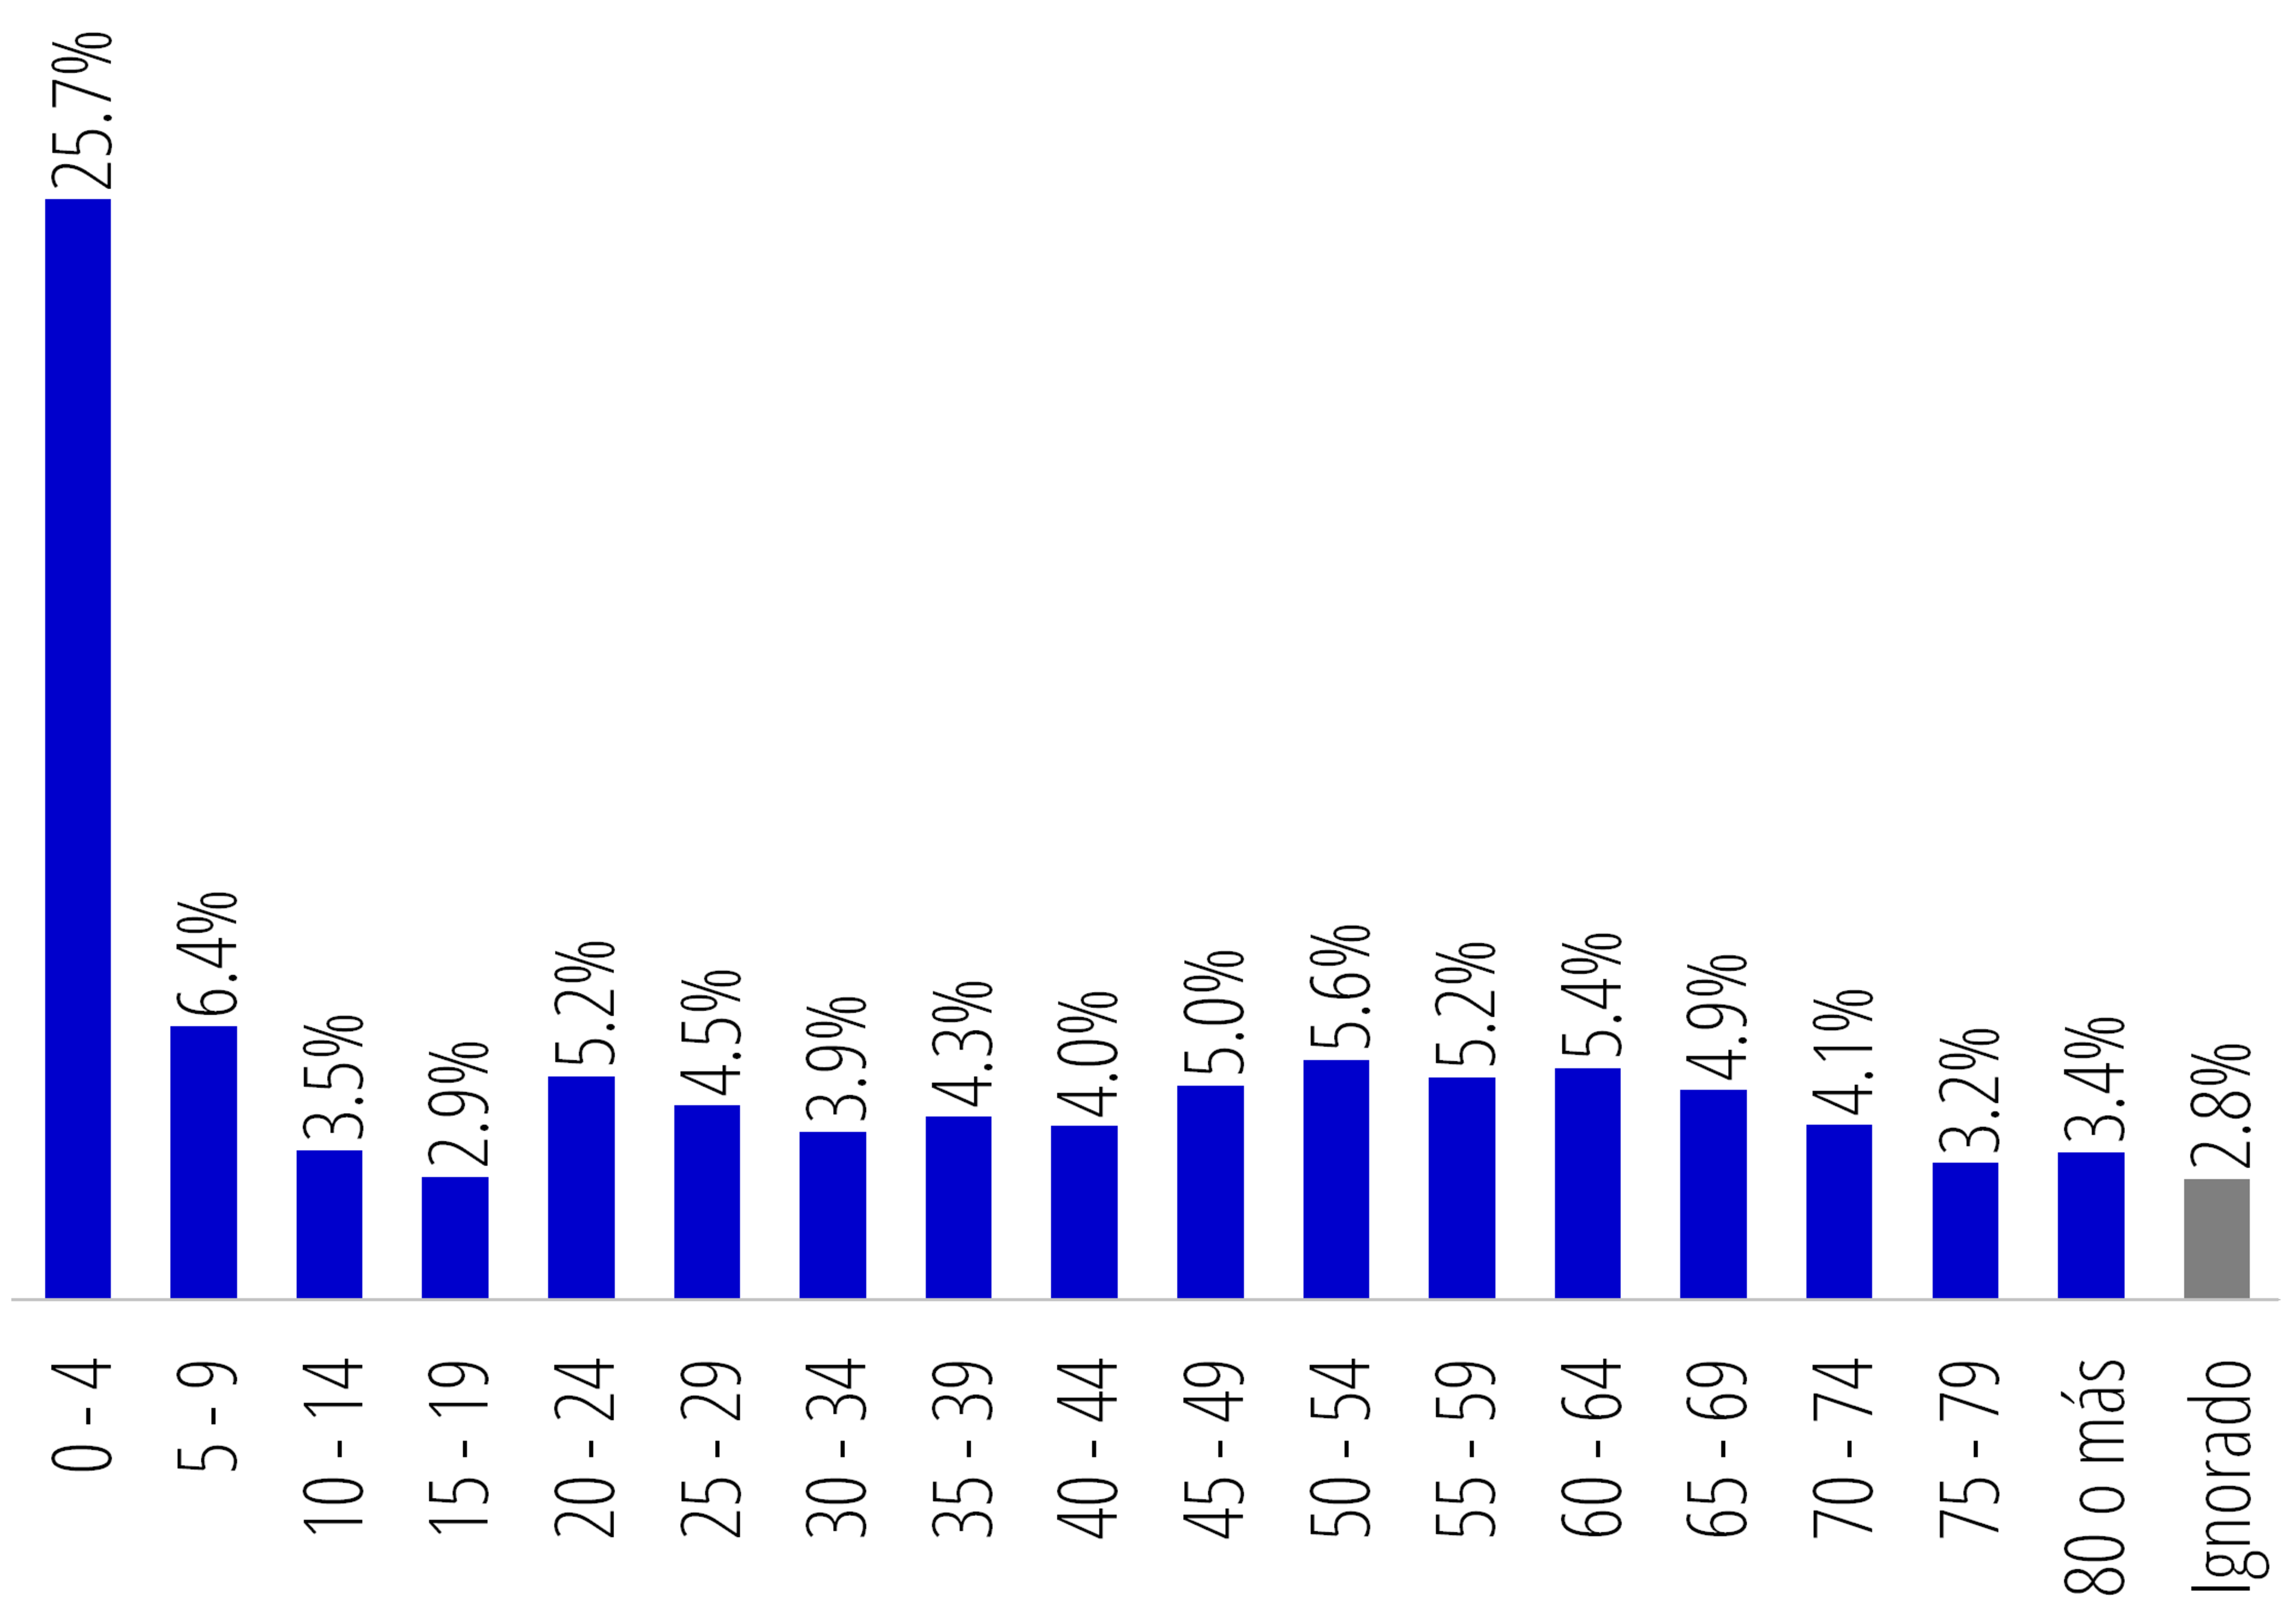
\includegraphics[width=32\cuadri]{plot.pdf}}{Aquí va la fuente.}{J4.10}

\cajitatabla{Hoho en la sección}{Ésta es la descripción, que si continúa, puede observarse que no alinea perfecto con el número de sección}{Titulín de gráfica}{         }{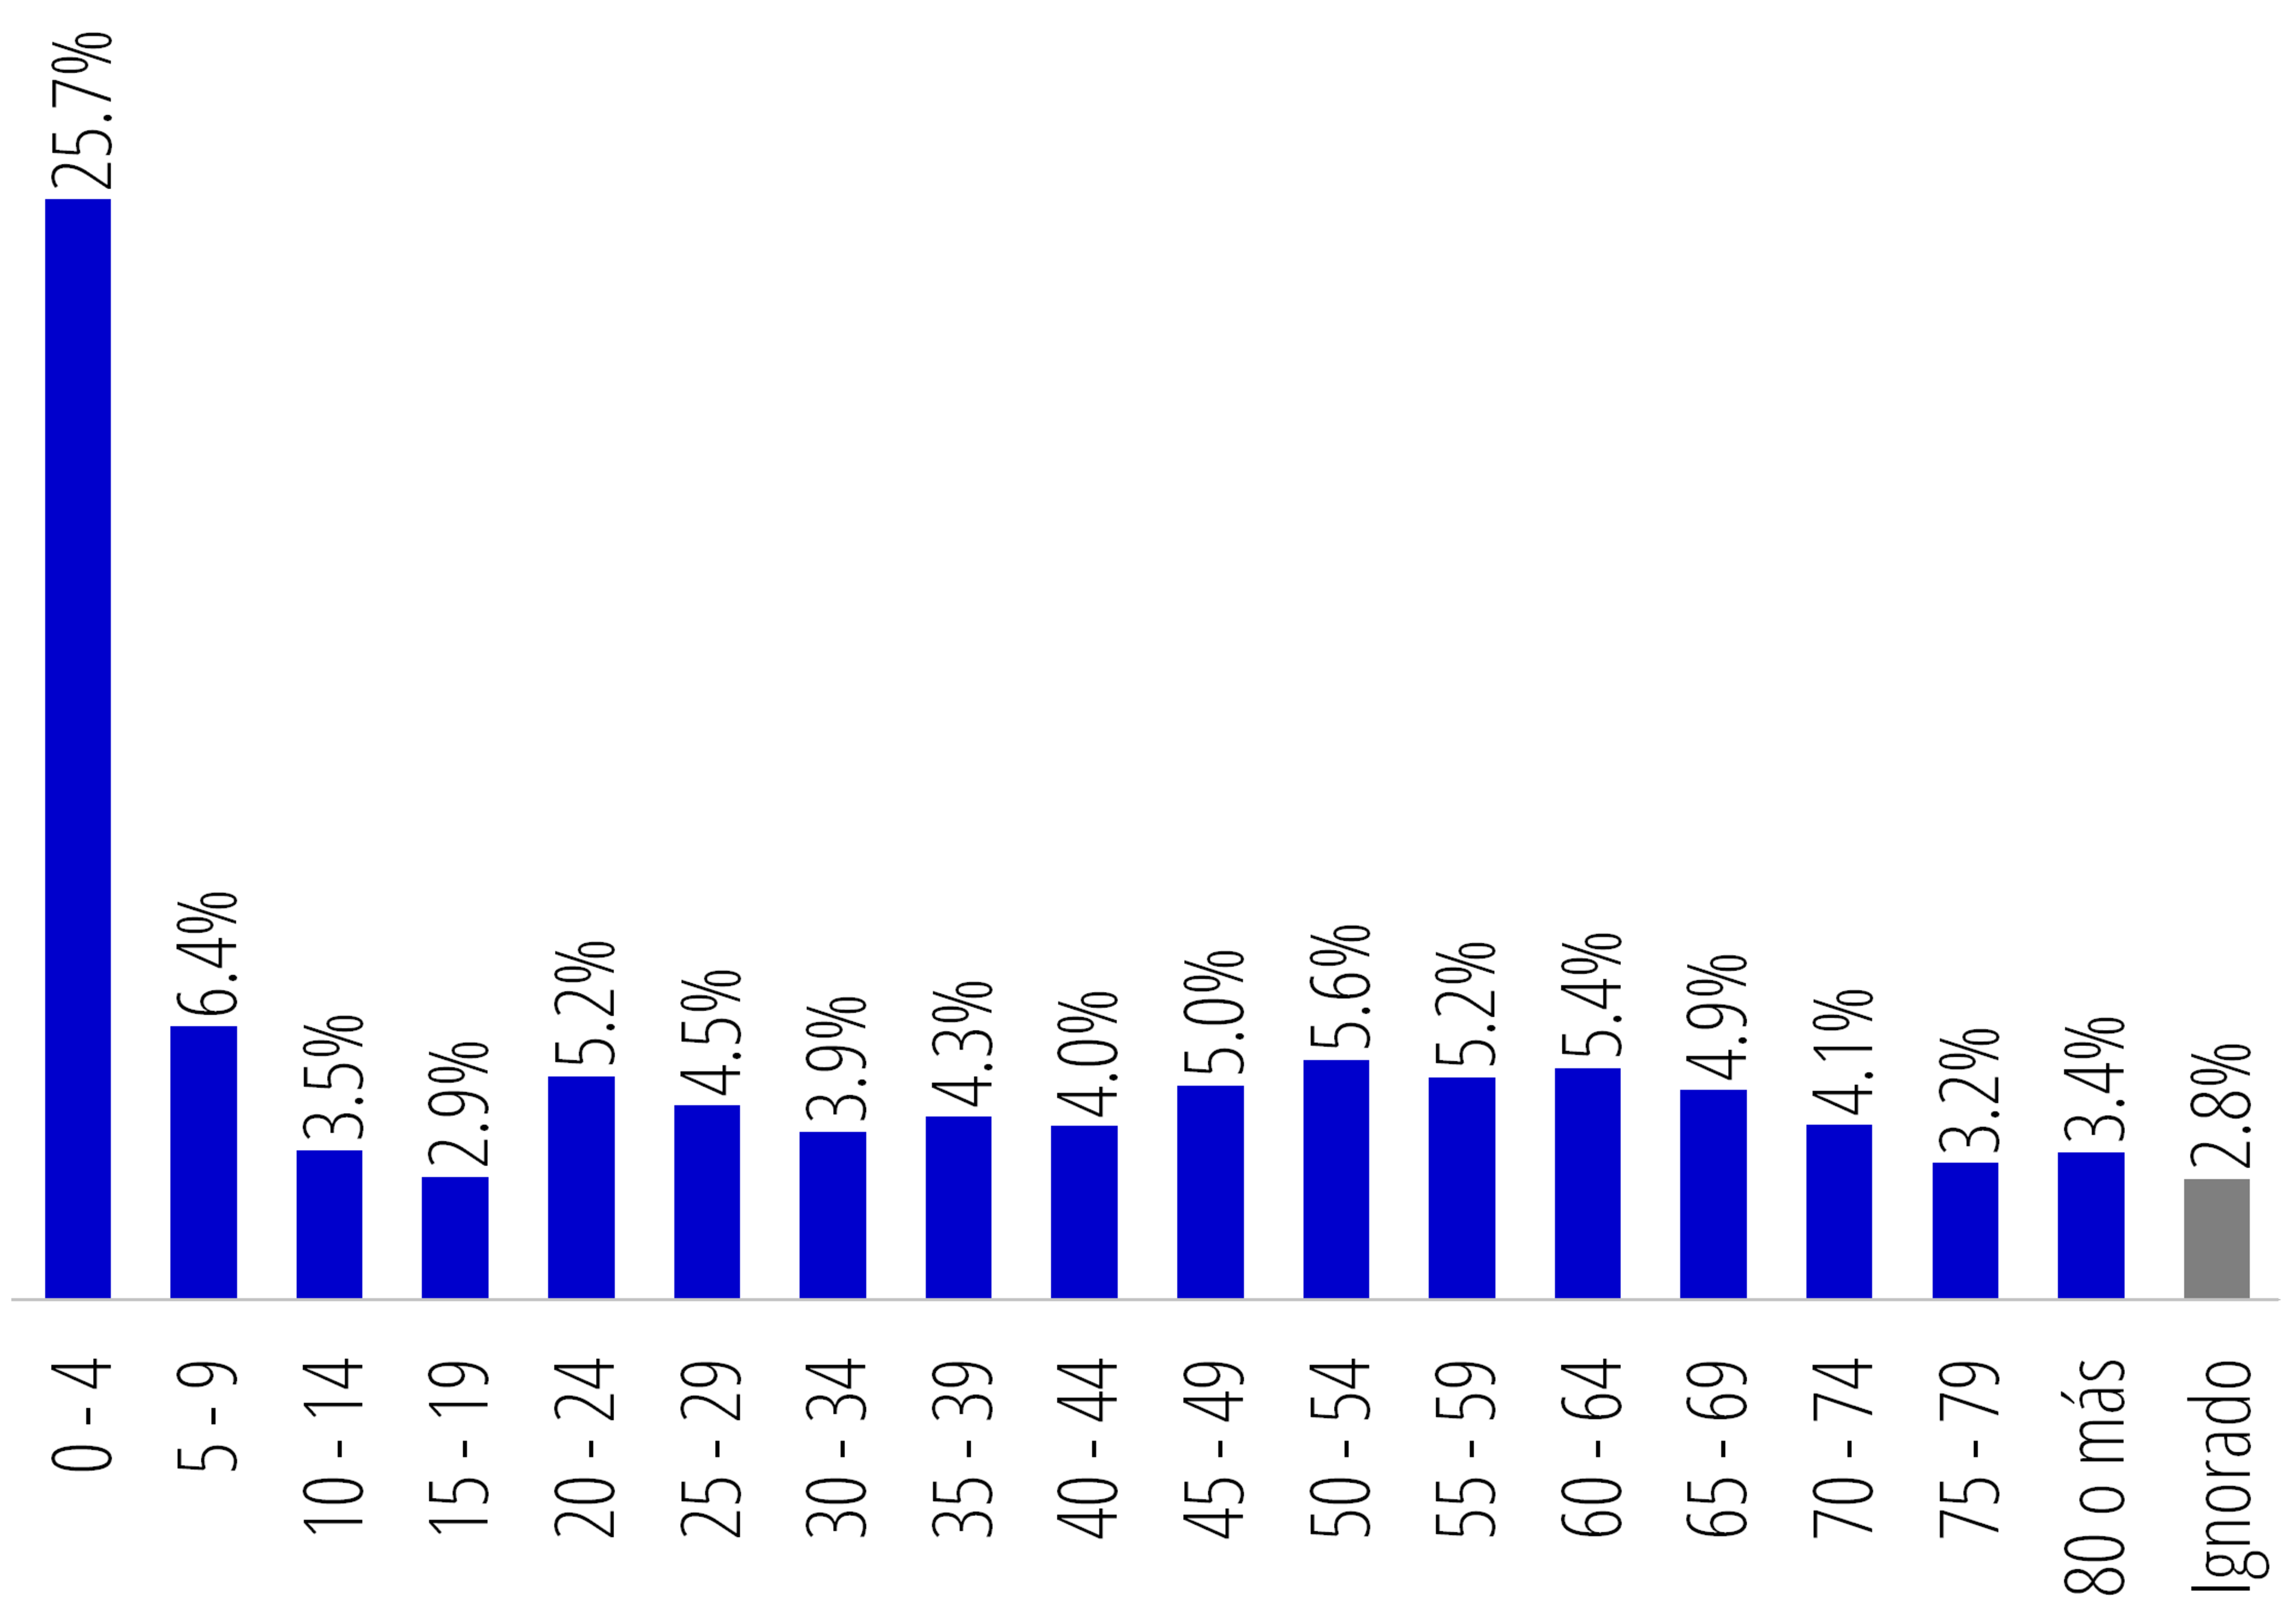
\includegraphics[width=32\cuadri]{plot.pdf}}{Aquí va la fuente.}



\cajotatabla{Título de la sección}{Aquí va el texto que describe a la tabla\footnote{Prueba de footnote}}{Título tabla}{}{ \ra{1.3}
		\begin{tabular}{rlrrrcc}
			&  \multicolumn{2}{c}{Número Índice} \phantom{abc} &   \multicolumn{4}{c}{Variación porcentual}\\
			\cline{2-3} \cline{5-7}
			Año &  Mes &  Índice & &  Mensual &  Acumulada&  Interanual\\ \midrule
			2014    &    Marzo    &    112.40    &    &    0.22 && \\ \bottomrule
		\end{tabular}
	}{Aquí va la fuente jojo.}
	
\cajotatabla{Título de la sección}{Aquí va el texto que describe a la tabla\footnote{Prueba de footnote}}{Título tabla}{}{ \ra{1.3}
	\begin{tabular}{rlrrrcc}
		&  \multicolumn{2}{c}{Número Índice} \phantom{abc} &   \multicolumn{4}{c}{Variación porcentual}\\
		\cline{2-3} \cline{5-7}
		Año &  Mes &  Índice & &  Mensual &  Acumulada&  Interanual\\ \midrule
		2014    &    Marzo    &    112.40    &    &    0.22 && \\ \bottomrule
	\end{tabular}
}{Aquí va la fuente jojo.}

\cajotatabla{Título de la sección}{Aquí va el texto que describe a la tabla\footnote{Prueba de footnote}}{Título tabla}{}{ \ra{1.3}
	\begin{tabular}{rlrrrcc}
		&  \multicolumn{2}{c}{Número Índice} \phantom{abc} &   \multicolumn{4}{c}{Variación porcentual}\\
		\cline{2-3} \cline{5-7}
		Año &  Mes &  Índice & &  Mensual &  Acumulada&  Interanual\\ \midrule
		2014    &    Marzo    &    112.40    &    &    0.22 && \\ \bottomrule
	\end{tabular}
}{Aquí va la fuente jojo.}

\cajotatabla{Título de la sección}{Aquí va el texto que describe a la tabla\footnote{Prueba de footnote}}{Título tabla}{}{ \ra{1.3}
	\begin{tabular}{rlrrrcc}
		&  \multicolumn{2}{c}{Número Índice} \phantom{abc} &   \multicolumn{4}{c}{Variación porcentual}\\
		\cline{2-3} \cline{5-7}
		Año &  Mes &  Índice & &  Mensual &  Acumulada&  Interanual\\ \midrule
		2014    &    Marzo    &    112.40    &    &    0.22 && \\ \bottomrule
	\end{tabular}
}{Aquí va la fuente jojo.}

\cajotatabla{Título de la sección}{Aquí va el texto que describe a la tabla\footnote{Prueba de footnote}}{Título tabla}{}{ \ra{1.3}
	\begin{tabular}{rlrrrcc}
		&  \multicolumn{2}{c}{Número Índice} \phantom{abc} &   \multicolumn{4}{c}{Variación porcentual}\\
		\cline{2-3} \cline{5-7}
		Año &  Mes &  Índice & &  Mensual &  Acumulada&  Interanual\\ \midrule
		2014    &    Marzo    &    112.40    &    &    0.22 && \\ \bottomrule
	\end{tabular}
}{Aquí va la fuente jojo.}

\cajotatabla{Título de la sección}{Aquí va el texto que describe a la tabla\footnote{Prueba de footnote}}{Título tabla}{}{ \ra{1.3}
	\begin{tabular}{rlrrrcc}
		&  \multicolumn{2}{c}{Número Índice} \phantom{abc} &   \multicolumn{4}{c}{Variación porcentual}\\
		\cline{2-3} \cline{5-7}
		Año &  Mes &  Índice & &  Mensual &  Acumulada&  Interanual\\ \midrule
		2014    &    Marzo    &    112.40    &    &    0.22 && \\ \bottomrule
	\end{tabular}
}{Aquí va la fuente jojo.}

\cajotatabla{Título de la sección}{Aquí va el texto que describe a la tabla\footnote{Prueba de footnote}}{Título tabla}{}{ \ra{1.3}
	\begin{tabular}{rlrrrcc}
		&  \multicolumn{2}{c}{Número Índice} \phantom{abc} &   \multicolumn{4}{c}{Variación porcentual}\\
		\cline{2-3} \cline{5-7}
		Año &  Mes &  Índice & &  Mensual &  Acumulada&  Interanual\\ \midrule
		2014    &    Marzo    &    112.40    &    &    0.22 && \\ \bottomrule
	\end{tabular}
}{Aquí va la fuente jojo.}


\cajotatabla{Título de la sección}{Aquí va el texto que describe a la tabla\footnote{Prueba de footnote}}{Título tabla}{}{ \ra{1.3}
	\begin{tabular}{rlrrrcc}
		&  \multicolumn{2}{c}{Número Índice} \phantom{abc} &   \multicolumn{4}{c}{Variación porcentual}\\
		\cline{2-3} \cline{5-7}
		Año &  Mes &  Índice & &  Mensual &  Acumulada&  Interanual\\ \midrule
		2014    &    Marzo    &    112.40    &    &    0.22 && \\ \bottomrule
	\end{tabular}
}{Aquí va la fuente jojo.}


\cajotatabla{Título de la sección}{Aquí va el texto que describe a la tabla\footnote{Prueba de footnote}}{Título tabla}{}{ \ra{1.3}
	\begin{tabular}{rlrrrcc}
		&  \multicolumn{2}{c}{Número Índice} \phantom{abc} &   \multicolumn{4}{c}{Variación porcentual}\\
		\cline{2-3} \cline{5-7}
		Año &  Mes &  Índice & &  Mensual &  Acumulada&  Interanual\\ \midrule
		2014    &    Marzo    &    112.40    &    &    0.22 && \\ \bottomrule
	\end{tabular}
}{Aquí va la fuente jojo.}


\cajotatabla{Título de la sección}{Aquí va el texto que describe a la tabla\footnote{Prueba de footnote}}{Título tabla}{}{ \ra{1.3}
	\begin{tabular}{rlrrrcc}
		&  \multicolumn{2}{c}{Número Índice} \phantom{abc} &   \multicolumn{4}{c}{Variación porcentual}\\
		\cline{2-3} \cline{5-7}
		Año &  Mes &  Índice & &  Mensual &  Acumulada&  Interanual\\ \midrule
		2014    &    Marzo    &    112.40    &    &    0.22 && \\ \bottomrule
	\end{tabular}
}{Aquí va la fuente jojo.}

\cajotatabla{Título de la sección}{Aquí va el texto que describe a la tabla\footnote{Prueba de footnote}}{Título tabla}{}{ \ra{1.3}
	\begin{tabular}{rlrrrcc}
		&  \multicolumn{2}{c}{Número Índice} \phantom{abc} &   \multicolumn{4}{c}{Variación porcentual}\\
		\cline{2-3} \cline{5-7}
		Año &  Mes &  Índice & &  Mensual &  Acumulada&  Interanual\\ \midrule
		2014    &    Marzo    &    112.40    &    &    0.22 && \\ \bottomrule
	\end{tabular}
}{Aquí va la fuente jojo.}


\cajotatabla{Título de la sección}{Aquí va el texto que describe a la tabla\footnote{Prueba de footnote}}{Título tabla}{}{ \ra{1.3}
	\begin{tabular}{rlrrrcc}
		&  \multicolumn{2}{c}{Número Índice} \phantom{abc} &   \multicolumn{4}{c}{Variación porcentual}\\
		\cline{2-3} \cline{5-7}
		Año &  Mes &  Índice & &  Mensual &  Acumulada&  Interanual\\ \midrule
		2014    &    Marzo    &    112.40    &    &    0.22 && \\ \bottomrule
	\end{tabular}
}{Aquí va la fuente jojo.}


\cajotatabla{Título de la sección}{Aquí va el texto que describe a la tabla\footnote{Prueba de footnote}}{Título tabla}{}{ \ra{1.3}
	\begin{tabular}{rlrrrcc}
		&  \multicolumn{2}{c}{Número Índice} \phantom{abc} &   \multicolumn{4}{c}{Variación porcentual}\\
		\cline{2-3} \cline{5-7}
		Año &  Mes &  Índice & &  Mensual &  Acumulada&  Interanual\\ \midrule
		2014    &    Marzo    &    112.40    &    &    0.22 && \\ \bottomrule
	\end{tabular}
}{Aquí va la fuente jojo.}

\cajotatabla{Título de la sección}{Aquí va el texto que describe a la tabla\footnote{Prueba de footnote}}{Título tabla}{}{ \ra{1.3}
	\begin{tabular}{rlrrrcc}
		&  \multicolumn{2}{c}{Número Índice} \phantom{abc} &   \multicolumn{4}{c}{Variación porcentual}\\
		\cline{2-3} \cline{5-7}
		Año &  Mes &  Índice & &  Mensual &  Acumulada&  Interanual\\ \midrule
		2014    &    Marzo    &    112.40    &    &    0.22 && \\ \bottomrule
	\end{tabular}
}{Aquí va la fuente jojo.}


\cajotatabla{Título de la sección}{Aquí va el texto que describe a la tabla\footnote{Prueba de footnote} La población ocupada se define como aquellas personas de 15 años o más que durante la semana de referencia hayan llevado a cabo, en un intervalo de al menos una hora, alguna actividad económica, trabajando en el período de referencia por un sueldo o salario en metálico o especie. También se incluye a personas que hayan estado ausentes temporalmente de su trabajo sin interrumpir su vínculo laboral con la unidad económica o empresa que lo contrata, es decir, con empleo pero sin trabajar.}{Título tabla}{Desagregación opcional}{LA TABLA EN CUESTIÓN}{Aquí va la fuente.}



\cajita[Hoho en el índice]{Título de caja largo wiri wiri Título de caja largo wiri wiri Título de caja largo wiri wiri }{\lipsum[4]}{Titulín de gráfica Titulín de gráfica Titulín de gráfica Titulín de gráfica Titulín de gráfica}{Desagregación de gráfica}{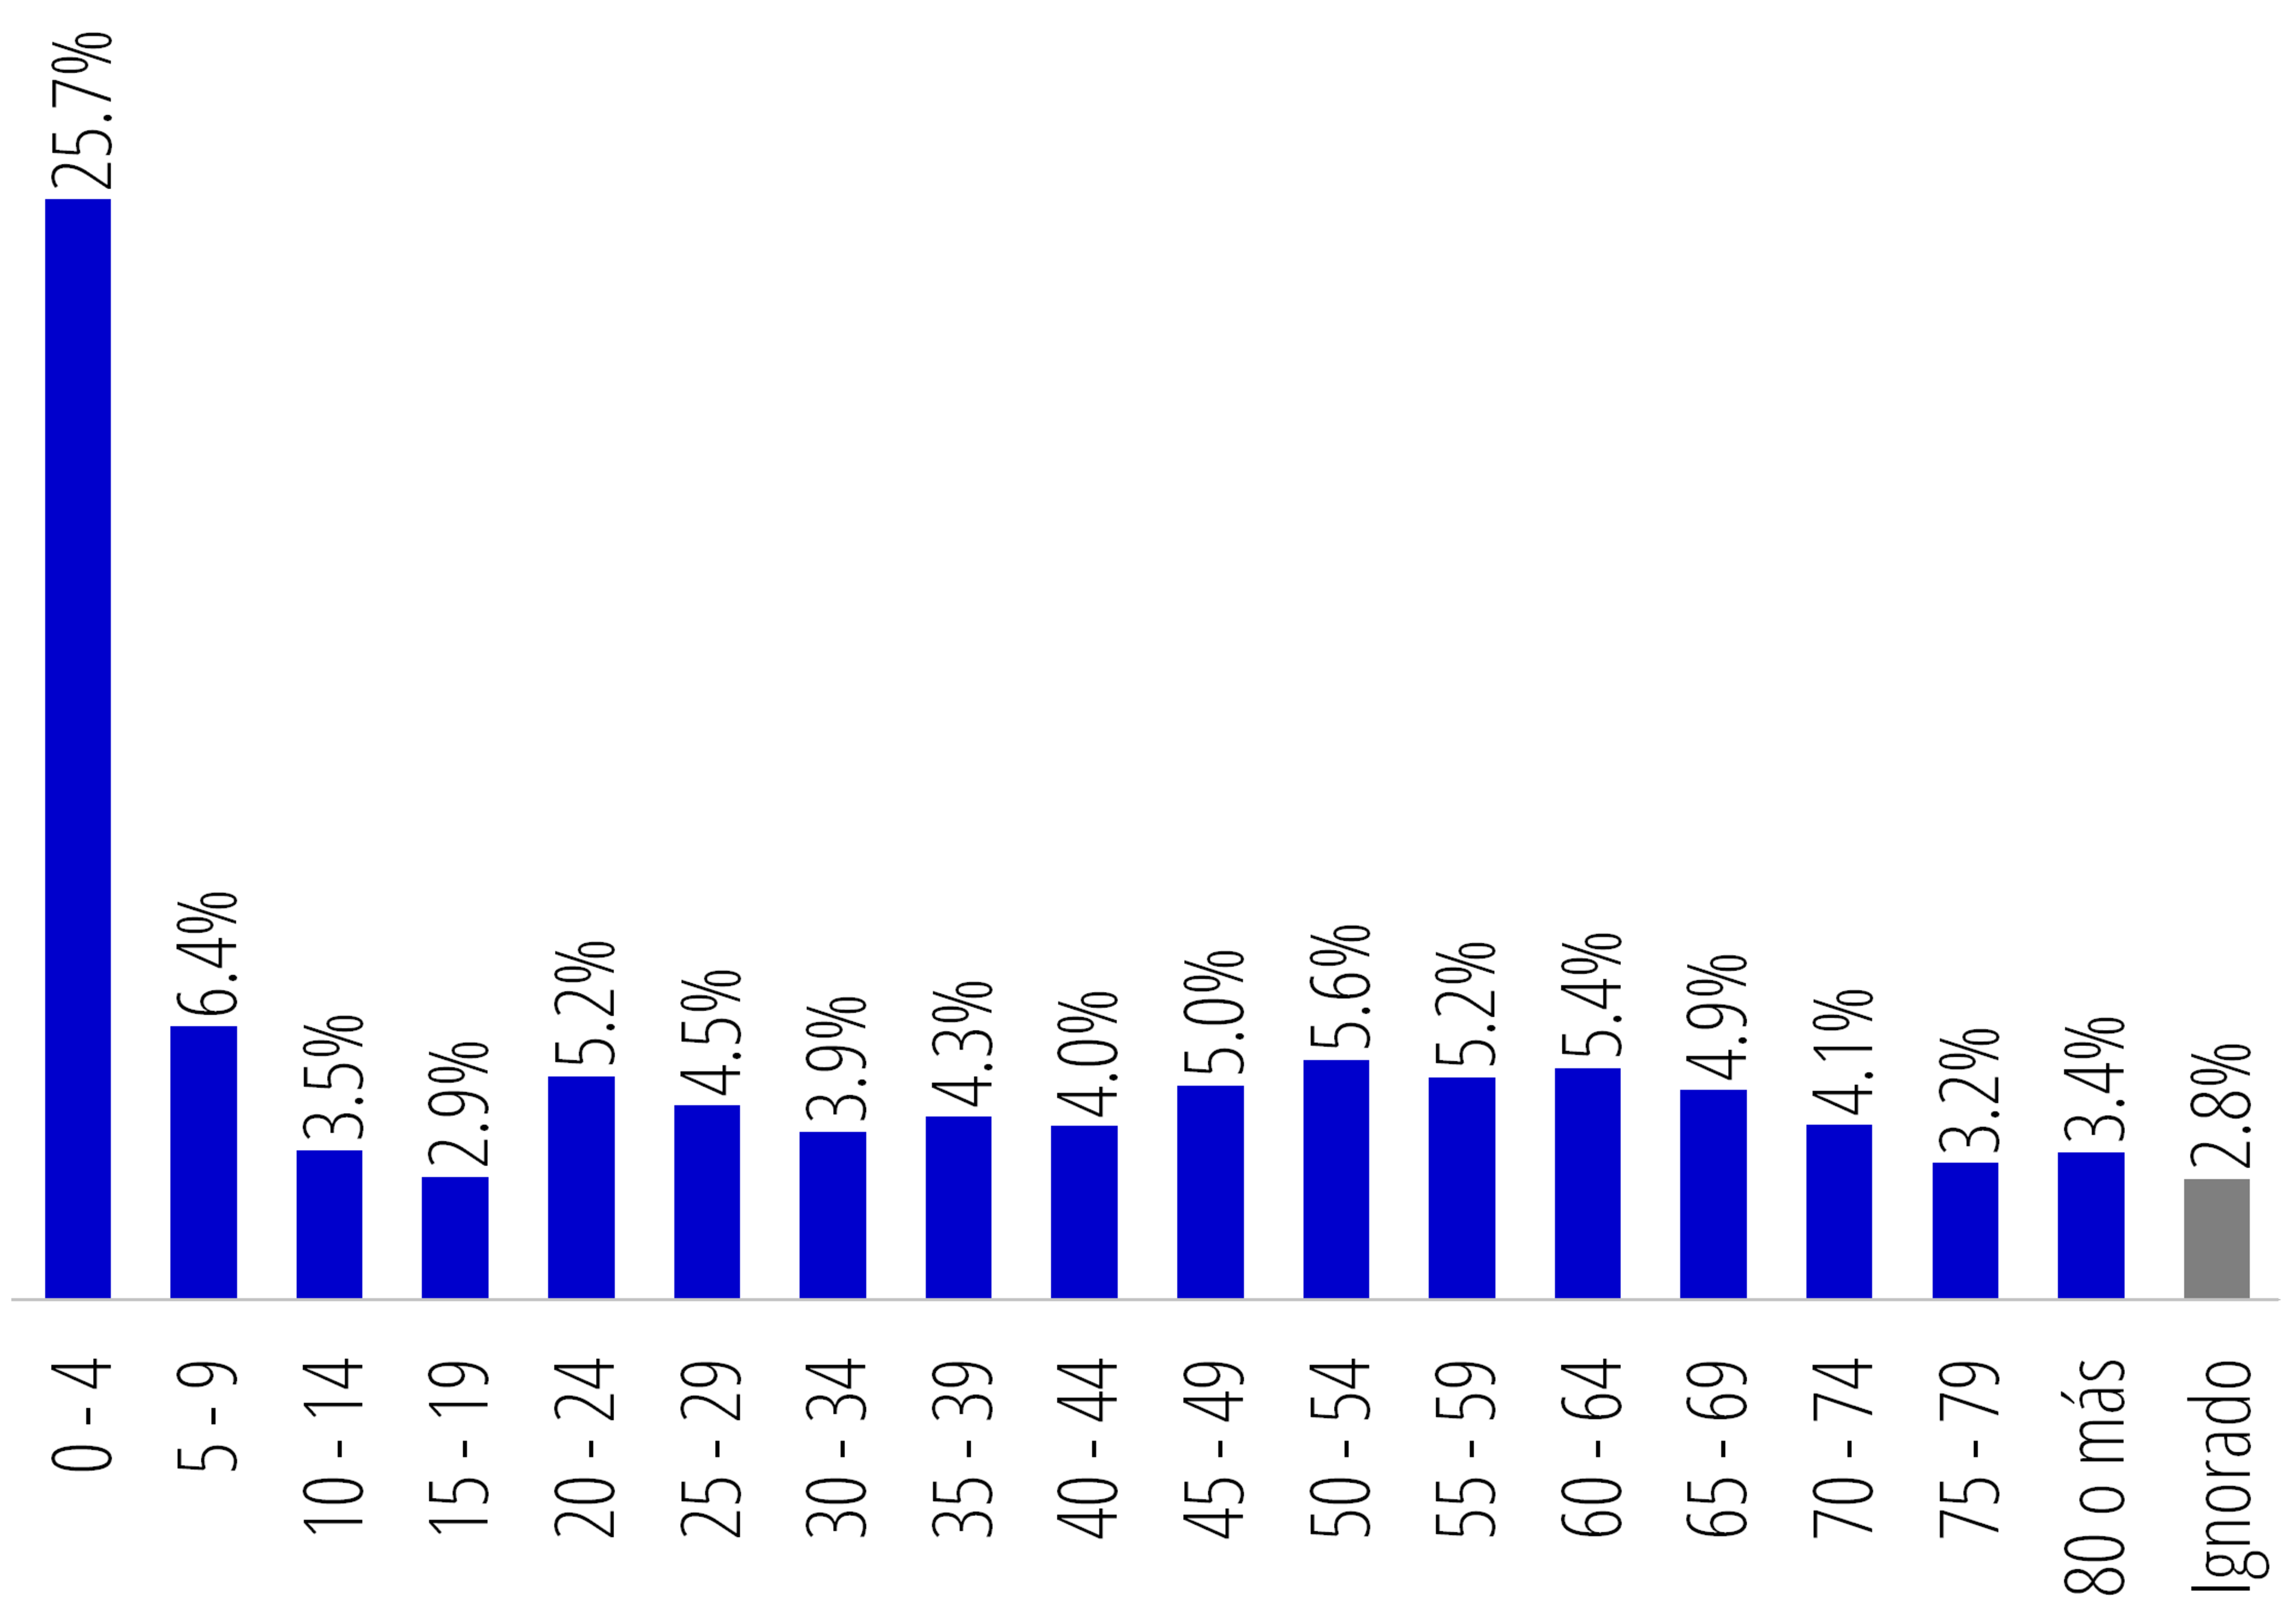
\includegraphics[width=32\cuadri]{plot.pdf}}{Aquí va la fuente.}

\INEchaptercarta{Capítulo dos}{Llegue...}

\cajita{Título de caja largo wiri wiri título de caja largo wiri wiri Título de caja largo wiri wiri }{\lipsum[1]}{Titulín de gráfica Titulín de gráfica Titulín de gráfica Titulín de gráfica Titulín de gráfica Titulín de gráfica}{Desagregación de gráfica}{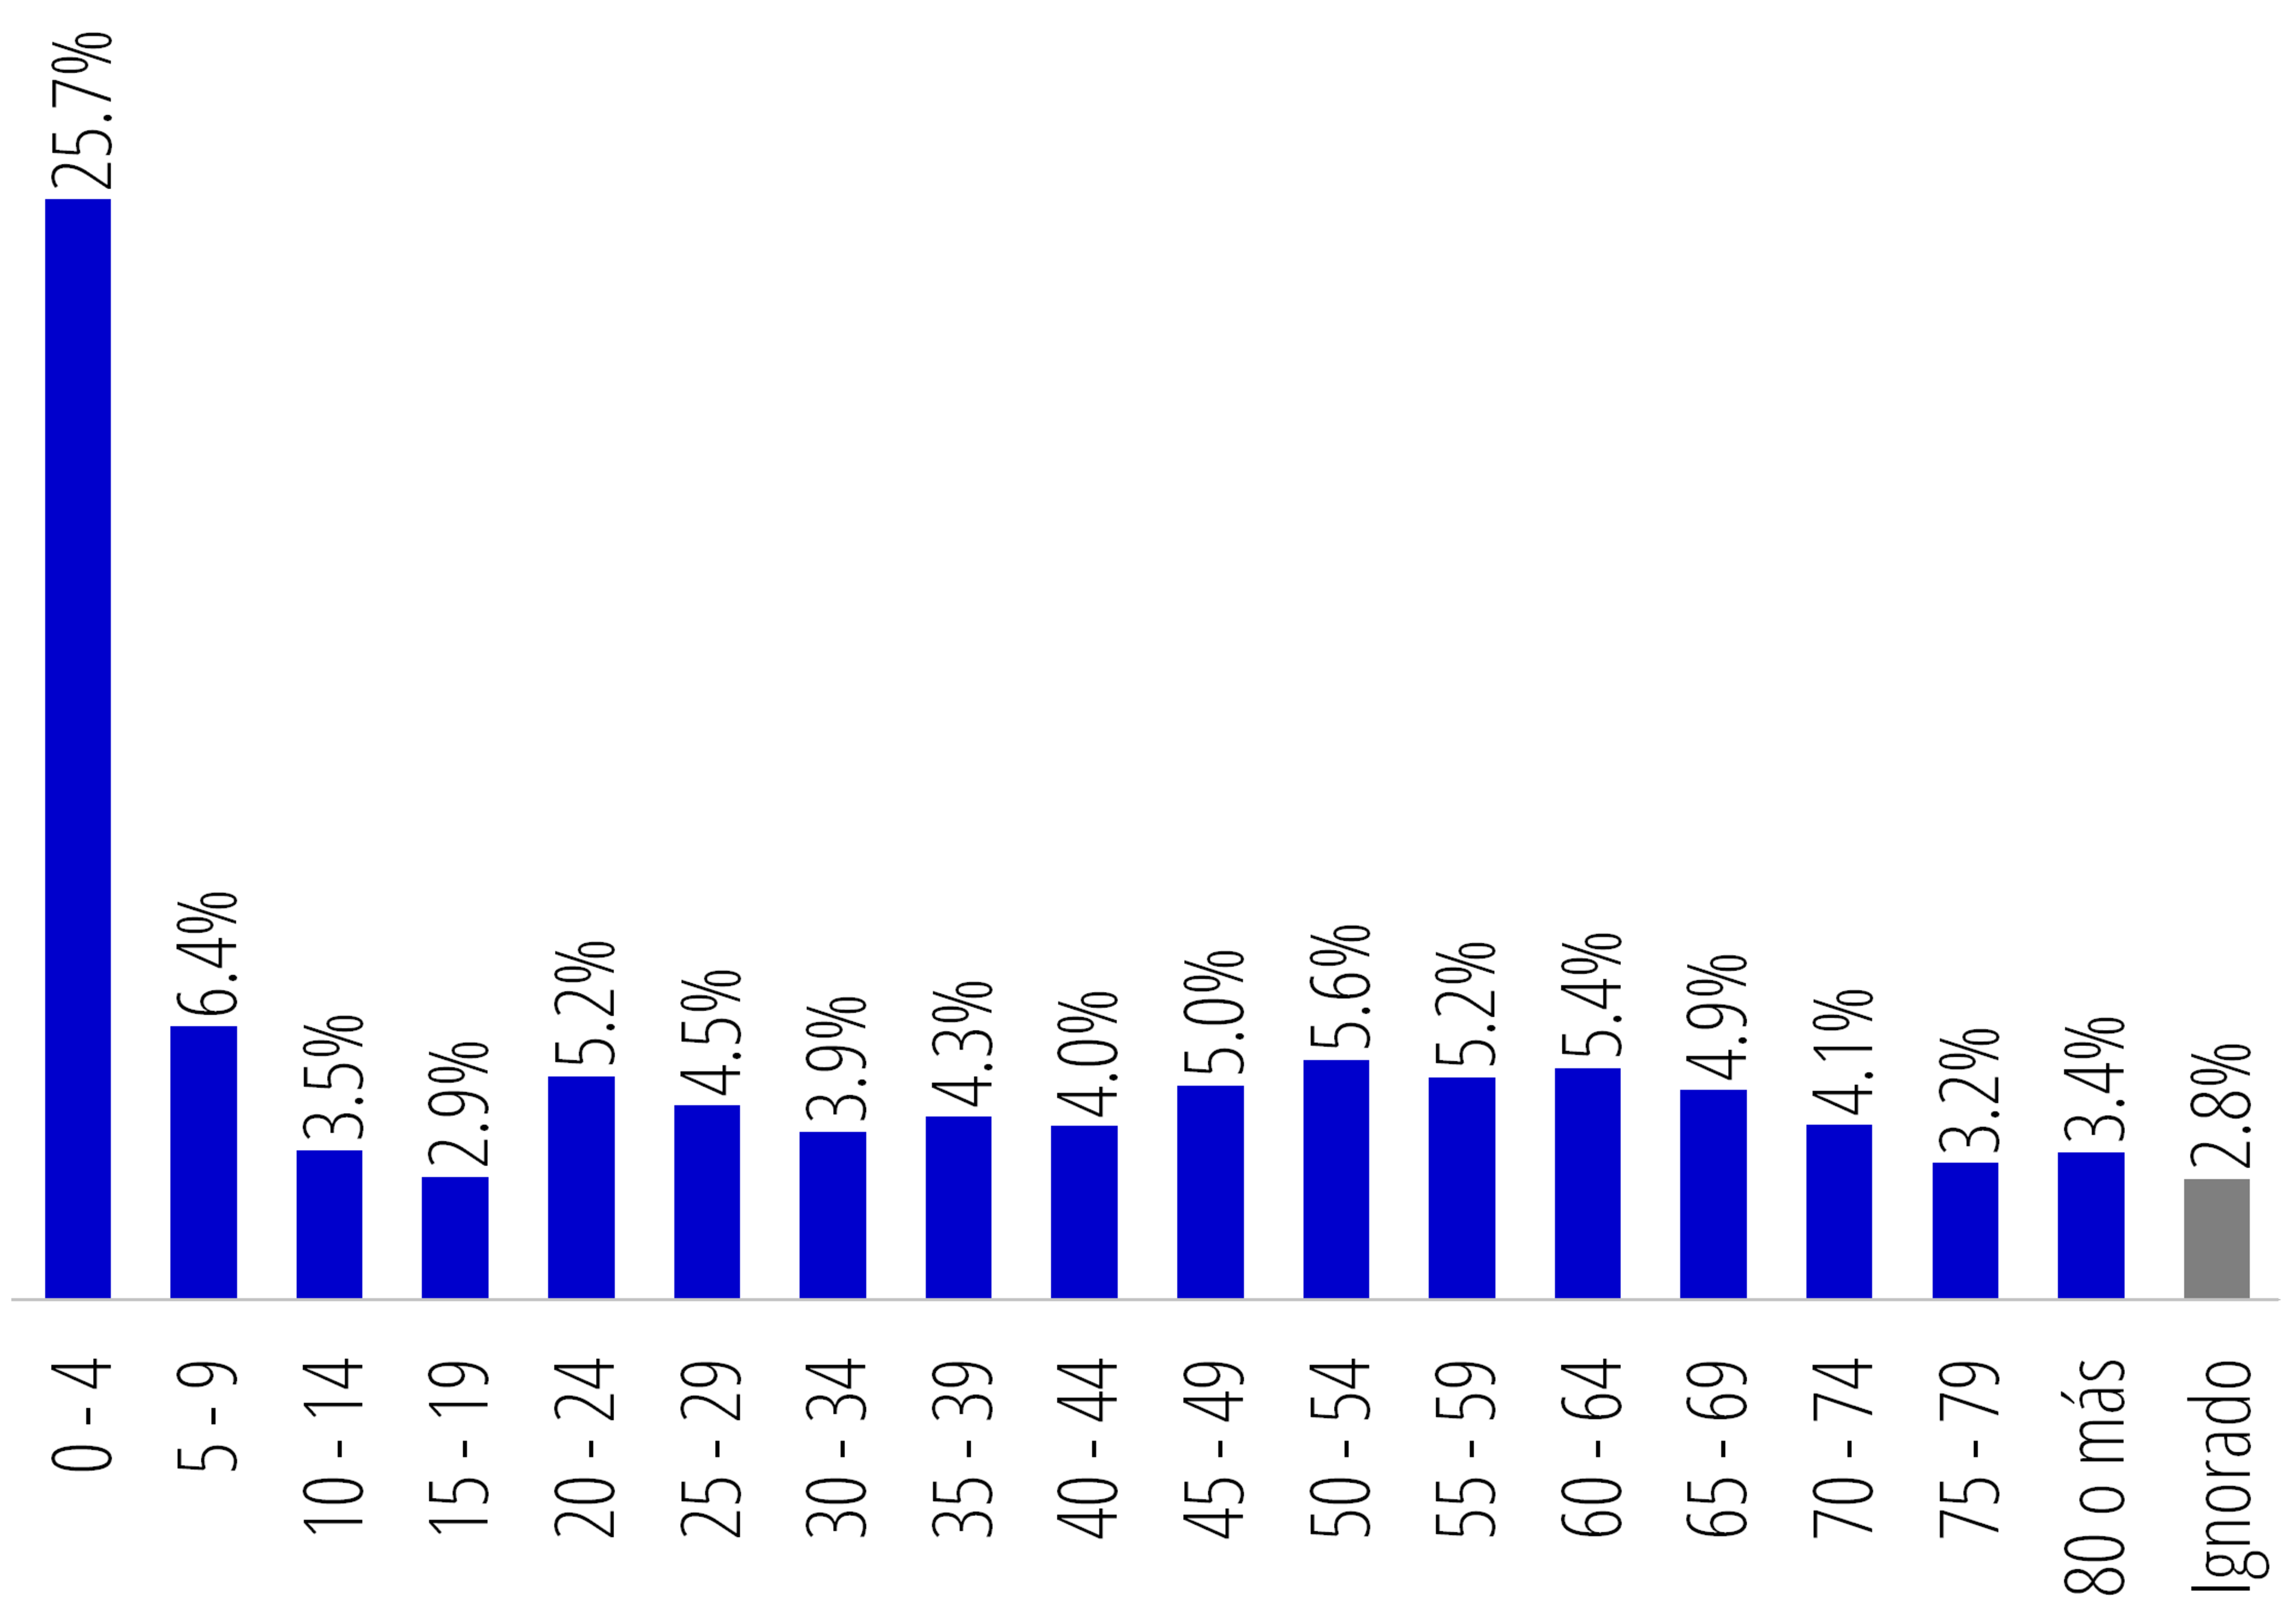
\includegraphics[width=32\cuadri]{plot.pdf}}{Aquí va la fuente.}
\cajita[Hoho en el índice]{Hoho en la sección}{\lipsum[4]

Hoho, esta es una prueba, revisando que todo funcione apropiadamente, tucuiri tucún y vuelta a probar.}{Titulín de gráfica}{Desagregación de gráfica}{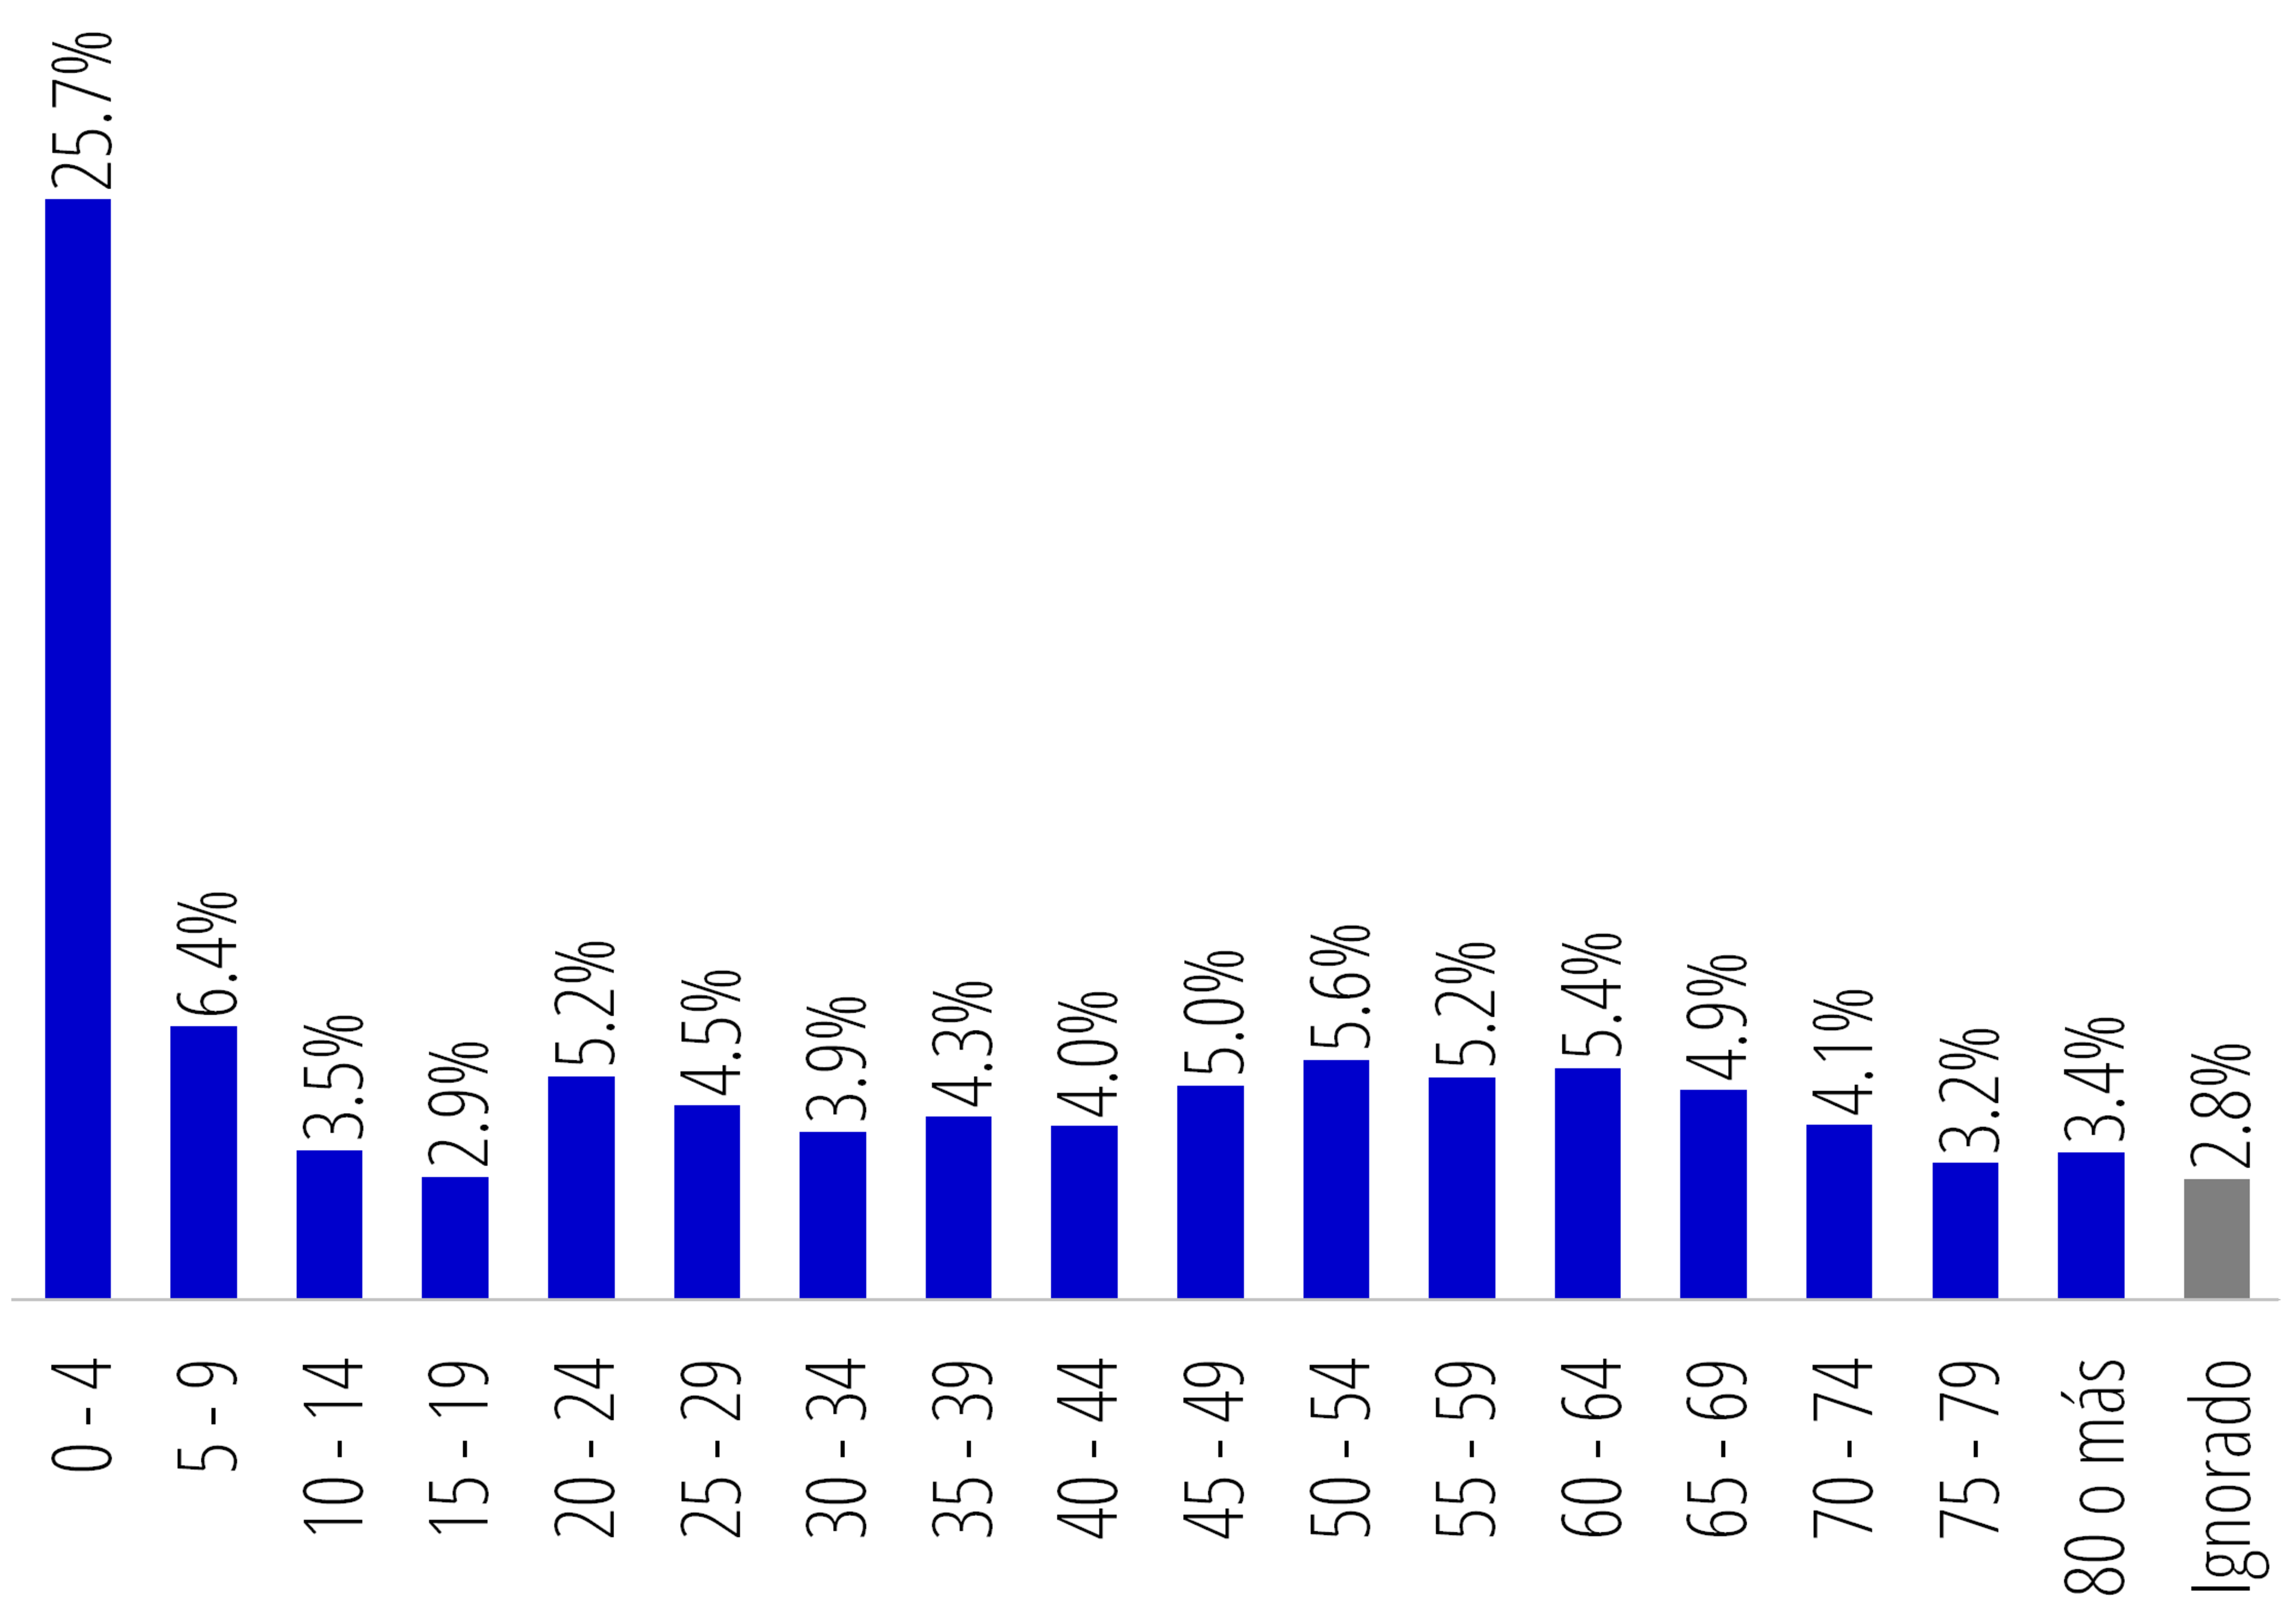
\includegraphics[width=32\cuadri]{plot.pdf}}{Aquí va la fuente.}

\INEpartecarta[Desglose]{Desglose por cajas y barritas coloridas}{\lipsum[4]}

\INEchaptercarta{Otro capítulo}{arg3}

\cajita{Hoho en la sección}{\lipsum[3]}{Titulín de gráfica}{Desagregación de gráfica}{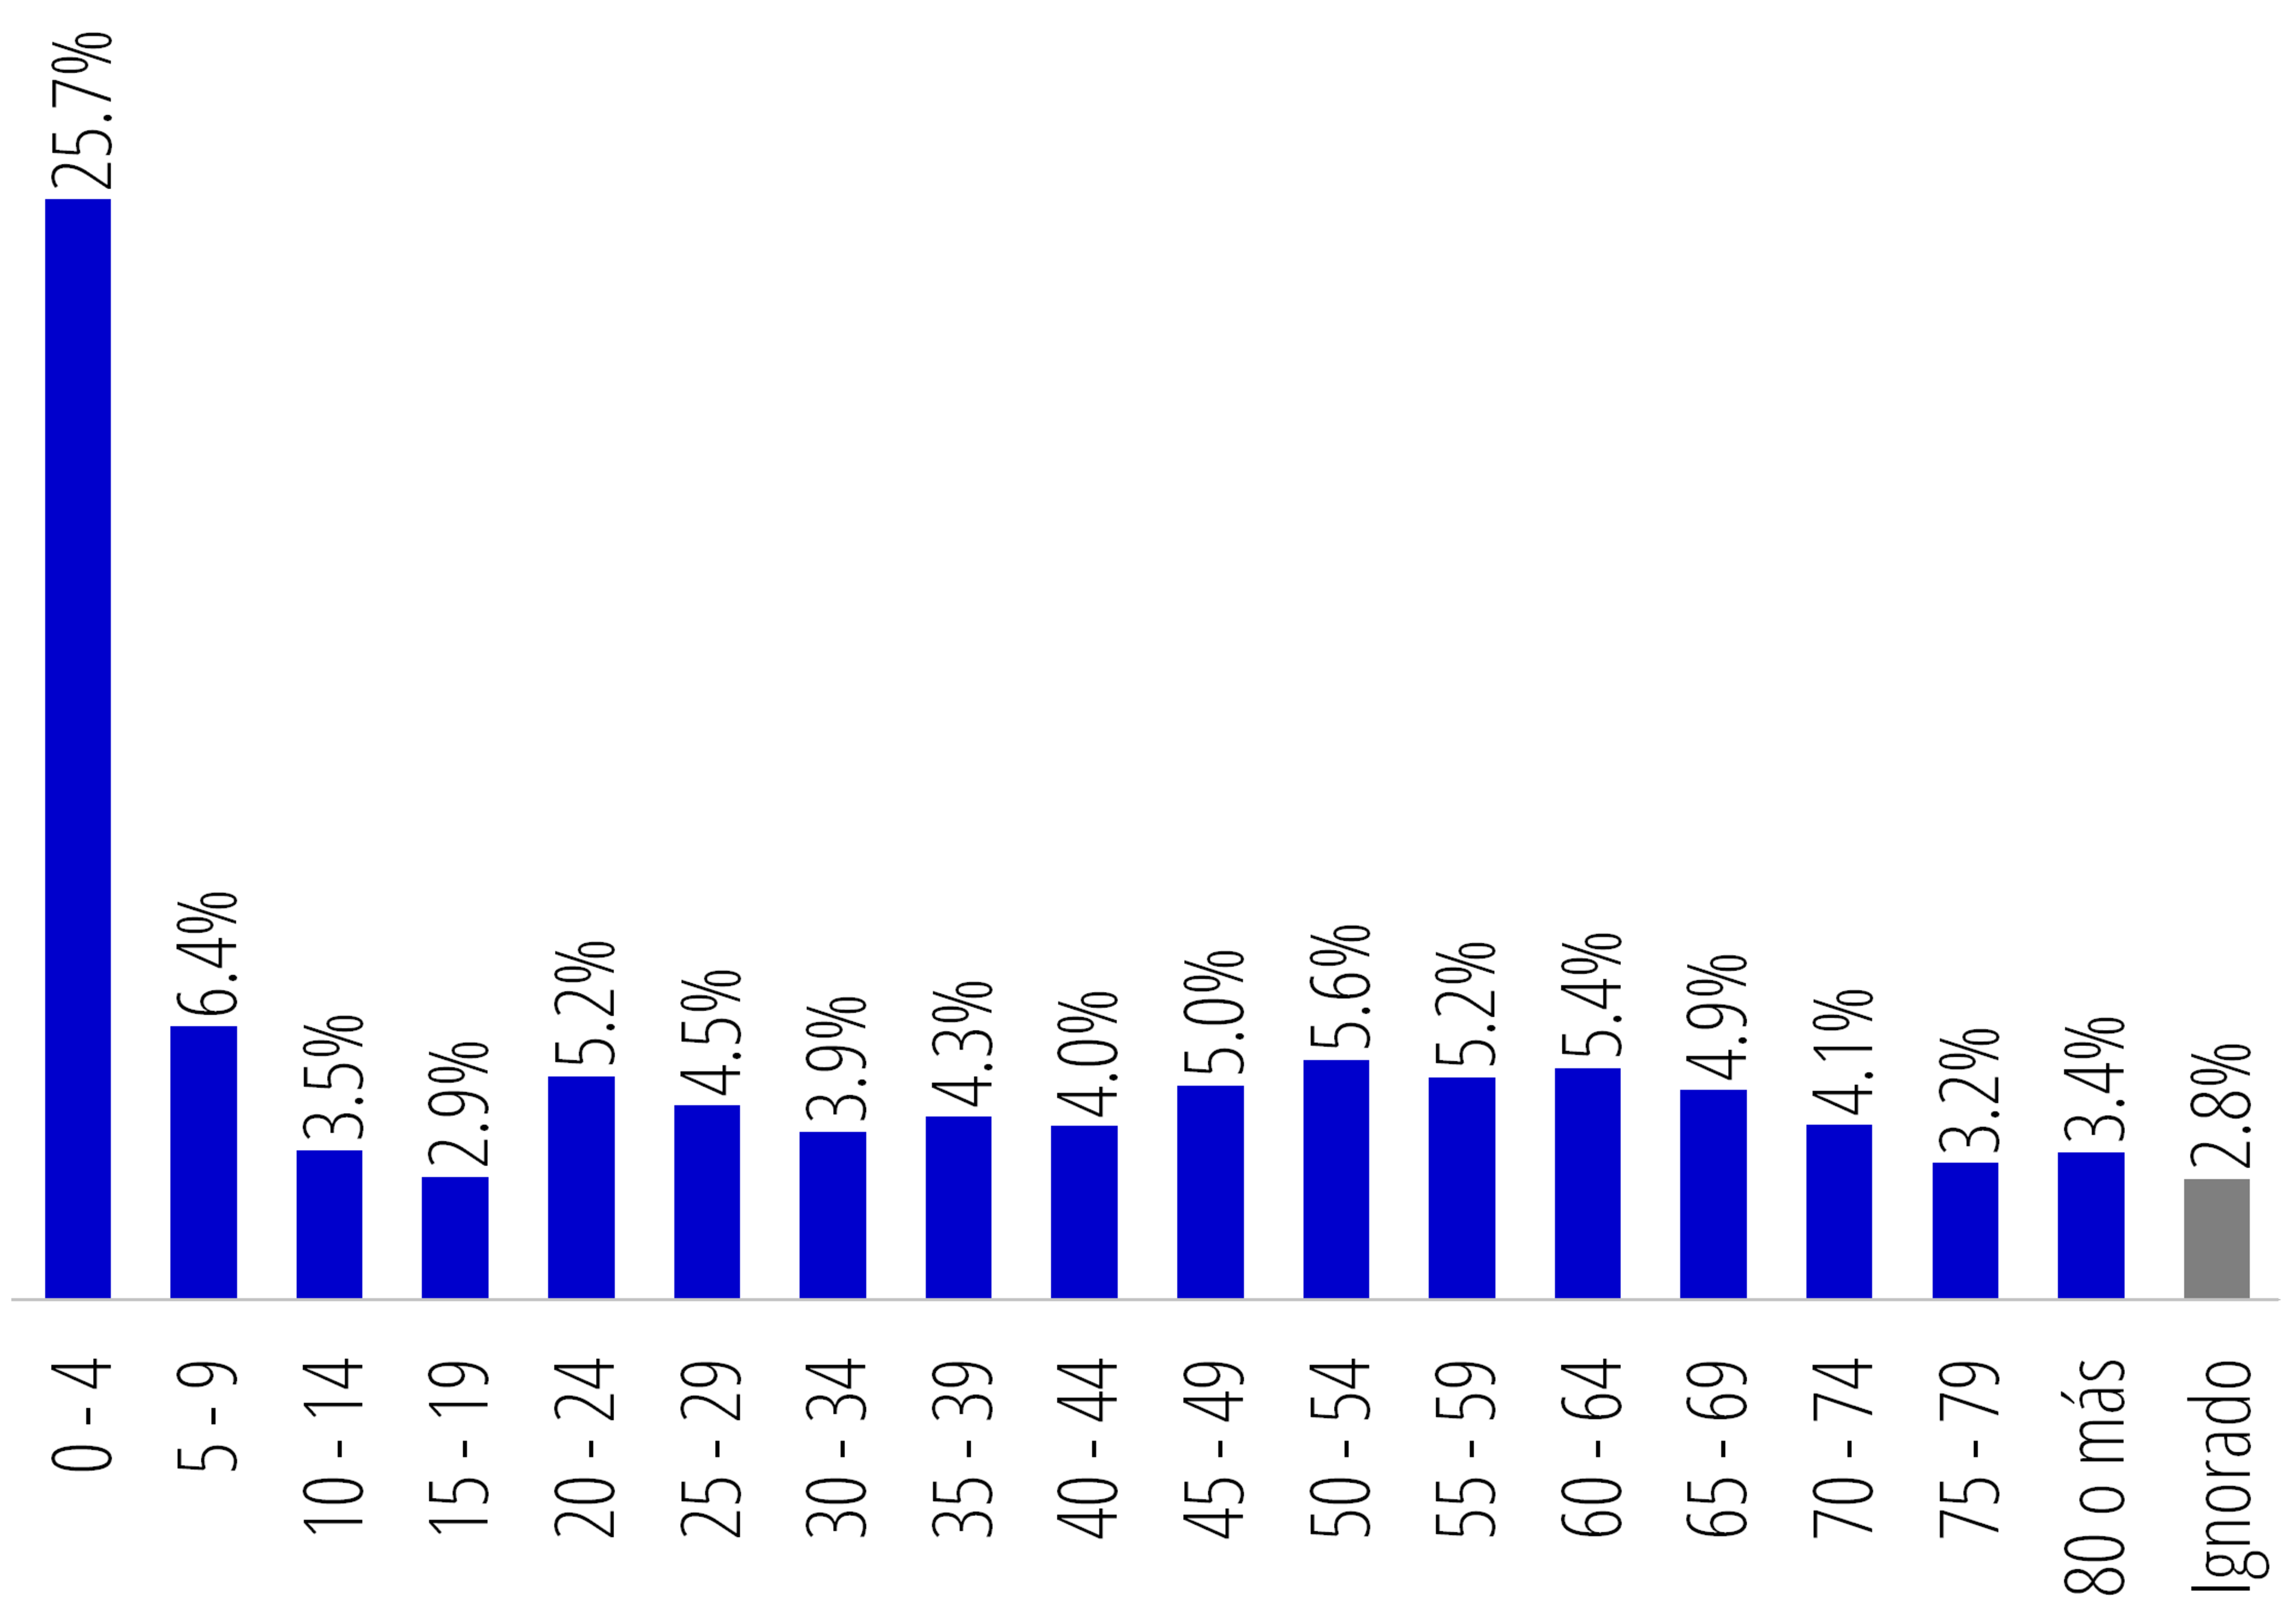
\includegraphics[width=32\cuadri]{plot.pdf}}{Aquí va la fuente.}



\cajotatabla{Título de la sección}{Aquí va el texto que describe a la tabla\footnote{Prueba de footnote}}{Título tabla}{}{ \ra{1.3}
	\begin{tabular}{rlrrrcc}
		&  \multicolumn{2}{c}{Número Índice} \phantom{abc} &   \multicolumn{4}{c}{Variación porcentual}\\
		\cline{2-3} \cline{5-7}
		Año &  Mes &  Índice & &  Mensual &  Acumulada&  Interanual\\ \midrule
		2014    &    Marzo    &    112.40    &    &    0.22 && \\ \bottomrule
	\end{tabular}
}{Aquí va la fuente jojo.}


\cajotatabla{Título de la sección}{Aquí va el texto que describe a la tabla\footnote{Prueba de footnote}}{Título tabla}{}{ \ra{1.3}
	\begin{tabular}{rlrrrcc}
		&  \multicolumn{2}{c}{Número Índice} \phantom{abc} &   \multicolumn{4}{c}{Variación porcentual}\\
		\cline{2-3} \cline{5-7}
		Año &  Mes &  Índice & &  Mensual &  Acumulada&  Interanual\\ \midrule
		2014    &    Marzo    &    112.40    &    &    0.22 && \\ \bottomrule
	\end{tabular}
}{Aquí va la fuente jojo.}

\cajotatabla{Título de la sección}{Aquí va el texto que describe a la tabla\footnote{Prueba de footnote}}{Título tabla}{}{ \ra{1.3}
	\begin{tabular}{rlrrrcc}
		&  \multicolumn{2}{c}{Número Índice} \phantom{abc} &   \multicolumn{4}{c}{Variación porcentual}\\
		\cline{2-3} \cline{5-7}
		Año &  Mes &  Índice & &  Mensual &  Acumulada&  Interanual\\ \midrule
		2014    &    Marzo    &    112.40    &    &    0.22 && \\ \bottomrule
	\end{tabular}
}{Aquí va la fuente jojo.}

\cajotatabla{Título de la sección}{Aquí va el texto que describe a la tabla\footnote{Prueba de footnote}}{Título tabla}{}{ \ra{1.3}
	\begin{tabular}{rlrrrcc}
		&  \multicolumn{2}{c}{Número Índice} \phantom{abc} &   \multicolumn{4}{c}{Variación porcentual}\\
		\cline{2-3} \cline{5-7}
		Año &  Mes &  Índice & &  Mensual &  Acumulada&  Interanual\\ \midrule
		2014    &    Marzo    &    112.40    &    &    0.22 && \\ \bottomrule
	\end{tabular}
}{Aquí va la fuente jojo.}

\cajotatabla{Título de la sección}{Aquí va el texto que describe a la tabla\footnote{Prueba de footnote}}{Título tabla}{}{ \ra{1.3}
	\begin{tabular}{rlrrrcc}
		&  \multicolumn{2}{c}{Número Índice} \phantom{abc} &   \multicolumn{4}{c}{Variación porcentual}\\
		\cline{2-3} \cline{5-7}
		Año &  Mes &  Índice & &  Mensual &  Acumulada&  Interanual\\ \midrule
		2014    &    Marzo    &    112.40    &    &    0.22 && \\ \bottomrule
	\end{tabular}
}{Aquí va la fuente jojo.}

\cajotatabla{Título de la sección}{Aquí va el texto que describe a la tabla\footnote{Prueba de footnote}}{Título tabla}{}{ \ra{1.3}
	\begin{tabular}{rlrrrcc}
		&  \multicolumn{2}{c}{Número Índice} \phantom{abc} &   \multicolumn{4}{c}{Variación porcentual}\\
		\cline{2-3} \cline{5-7}
		Año &  Mes &  Índice & &  Mensual &  Acumulada&  Interanual\\ \midrule
		2014    &    Marzo    &    112.40    &    &    0.22 && \\ \bottomrule
	\end{tabular}
}{Aquí va la fuente jojo.}


\cajotatabla{Prueba de título largo}{Aquí va el texto que describe a la tabla\footnote{Prueba de footnote}}{Consideremos un título de tabla o mapa que sea demasiado largo,\\ tan largo incluso que requiera de más de una línea}{Y para más, con desagregación}{ \ra{1.3}
	\begin{tabular}{rlrrrcc}
		&  \multicolumn{2}{c}{Número Índice} \phantom{abc} &   \multicolumn{4}{c}{Variación porcentual}\\
		\cline{2-3} \cline{5-7}
		Año &  Mes &  Índice & &  Mensual &  Acumulada&  Interanual\\ \midrule
		2014    &    Marzo    &    112.40    &    &    0.22 && \\ \bottomrule
	\end{tabular}
}{Aquí va la fuente jojo.}


\cajotatabla{Título de la sección}{Aquí va el texto que describe a la tabla\footnote{Prueba de footnote}}{Título tabla}{}{ \ra{1.3}
	\begin{tabular}{rlrrrcc}
		&  \multicolumn{2}{c}{Número Índice} \phantom{abc} &   \multicolumn{4}{c}{Variación porcentual}\\
		\cline{2-3} \cline{5-7}
		Año &  Mes &  Índice & &  Mensual &  Acumulada&  Interanual\\ \midrule
		2014    &    Marzo    &    112.40    &    &    0.22 && \\ \bottomrule
	\end{tabular}
}{Aquí va la fuente jojo.}


\cajotatabla{Título de la sección}{Aquí va el texto que describe a la tabla\footnote{Prueba de footnote}}{Título tabla}{}{ \ra{1.3}
	\begin{tabular}{rlrrrcc}
		&  \multicolumn{2}{c}{Número Índice} \phantom{abc} &   \multicolumn{4}{c}{Variación porcentual}\\
		\cline{2-3} \cline{5-7}
		Año &  Mes &  Índice & &  Mensual &  Acumulada&  Interanual\\ \midrule
		2014    &    Marzo    &    112.40    &    &    0.22 && \\ \bottomrule
	\end{tabular}
}{Aquí va la fuente jojo.}


\cajotatabla{Título de la sección}{Aquí va el texto que describe a la tabla\footnote{Prueba de footnote}}{Título tabla}{}{ \ra{1.3}
	\begin{tabular}{rlrrrcc}
		&  \multicolumn{2}{c}{Número Índice} \phantom{abc} &   \multicolumn{4}{c}{Variación porcentual}\\
		\cline{2-3} \cline{5-7}
		Año &  Mes &  Índice & &  Mensual &  Acumulada&  Interanual\\ \midrule
		2014    &    Marzo    &    112.40    &    &    0.22 && \\ \bottomrule
	\end{tabular}
}{Aquí va la fuente jojo.}


\noindent\begin{cajita-arriba}
\stepcounter{section}
\addcontentsline{toc}{section}{\numberline{\thesection} Sección de prueba}
\titulizador{Sección de prueba con un nombre muy largo para ver qué sucede cuando acontece lo que pasaría.}

\begin{tabular}[b]{@{}p{17.5\cuadri}@{}p{1.5\cuadri}@{} x{34\cuadri}@{}}
& &\\[0.5\cuadri]
\begin{descripcion-cajita}
\parskip 6pt\parindent 2em%
\textollamada[*]{\centering
$\!FGT(\alpha)= \frac{1}{N}\!\!\!\!\!\!\displaystyle\sum_{\begin{smallmatrix}\text{\fontsize{0.6mm}{1em} \selectfont $1\!\!\leq\!\! i\!\!\leq\!\! N$}\\[0.3mm]\text{\fontsize{0.6mm}{1em} \selectfont $x_i\!\!<\!\!L\!P\!E$}\end{smallmatrix}}\!\!\!\!\! \left(1-\frac{x_i}{LPE}\right)^\alpha\!\!,\ \ \alpha=0\!$}
Chaleco, este es un ejemplo. de párrafo.  Debo escribir algunas líneas para corroborar que separa los párrafos adecuadamente.  Esto resulta interesante.

Chaleco viteh\llamada Ahora\textollamada{alusión a viteh.} debo\notita{alusión a debo. Pablito clavó un clavito en la calva de un calvito, tres tristes tigres tragaban trigo en un trigal. Mambrú se fue a la guerra que dolor que dolor que pena.} copiar y pegar. el párrafo anterior pero me da hueva,  Así que escribiré un poquito más\notita{alusión a poquito más}. Continuando la discusión latinezca podemos apreciar que tengo mucho sueño.  Pero esto no es nada nuevo para el lector.
\end{descripcion-cajita}
  & &
\begin{grafica-cajita}
\begin{center}
\textbf{Título de gráfica, que a veces puede\\ 
llegar a ser bastante largo}\\[-1pt]
{\footnotesize\texttwelveudash$\,\,$Desagregación de gráfica$\,\,$\texttwelveudash}\\[0.6\cuadri]
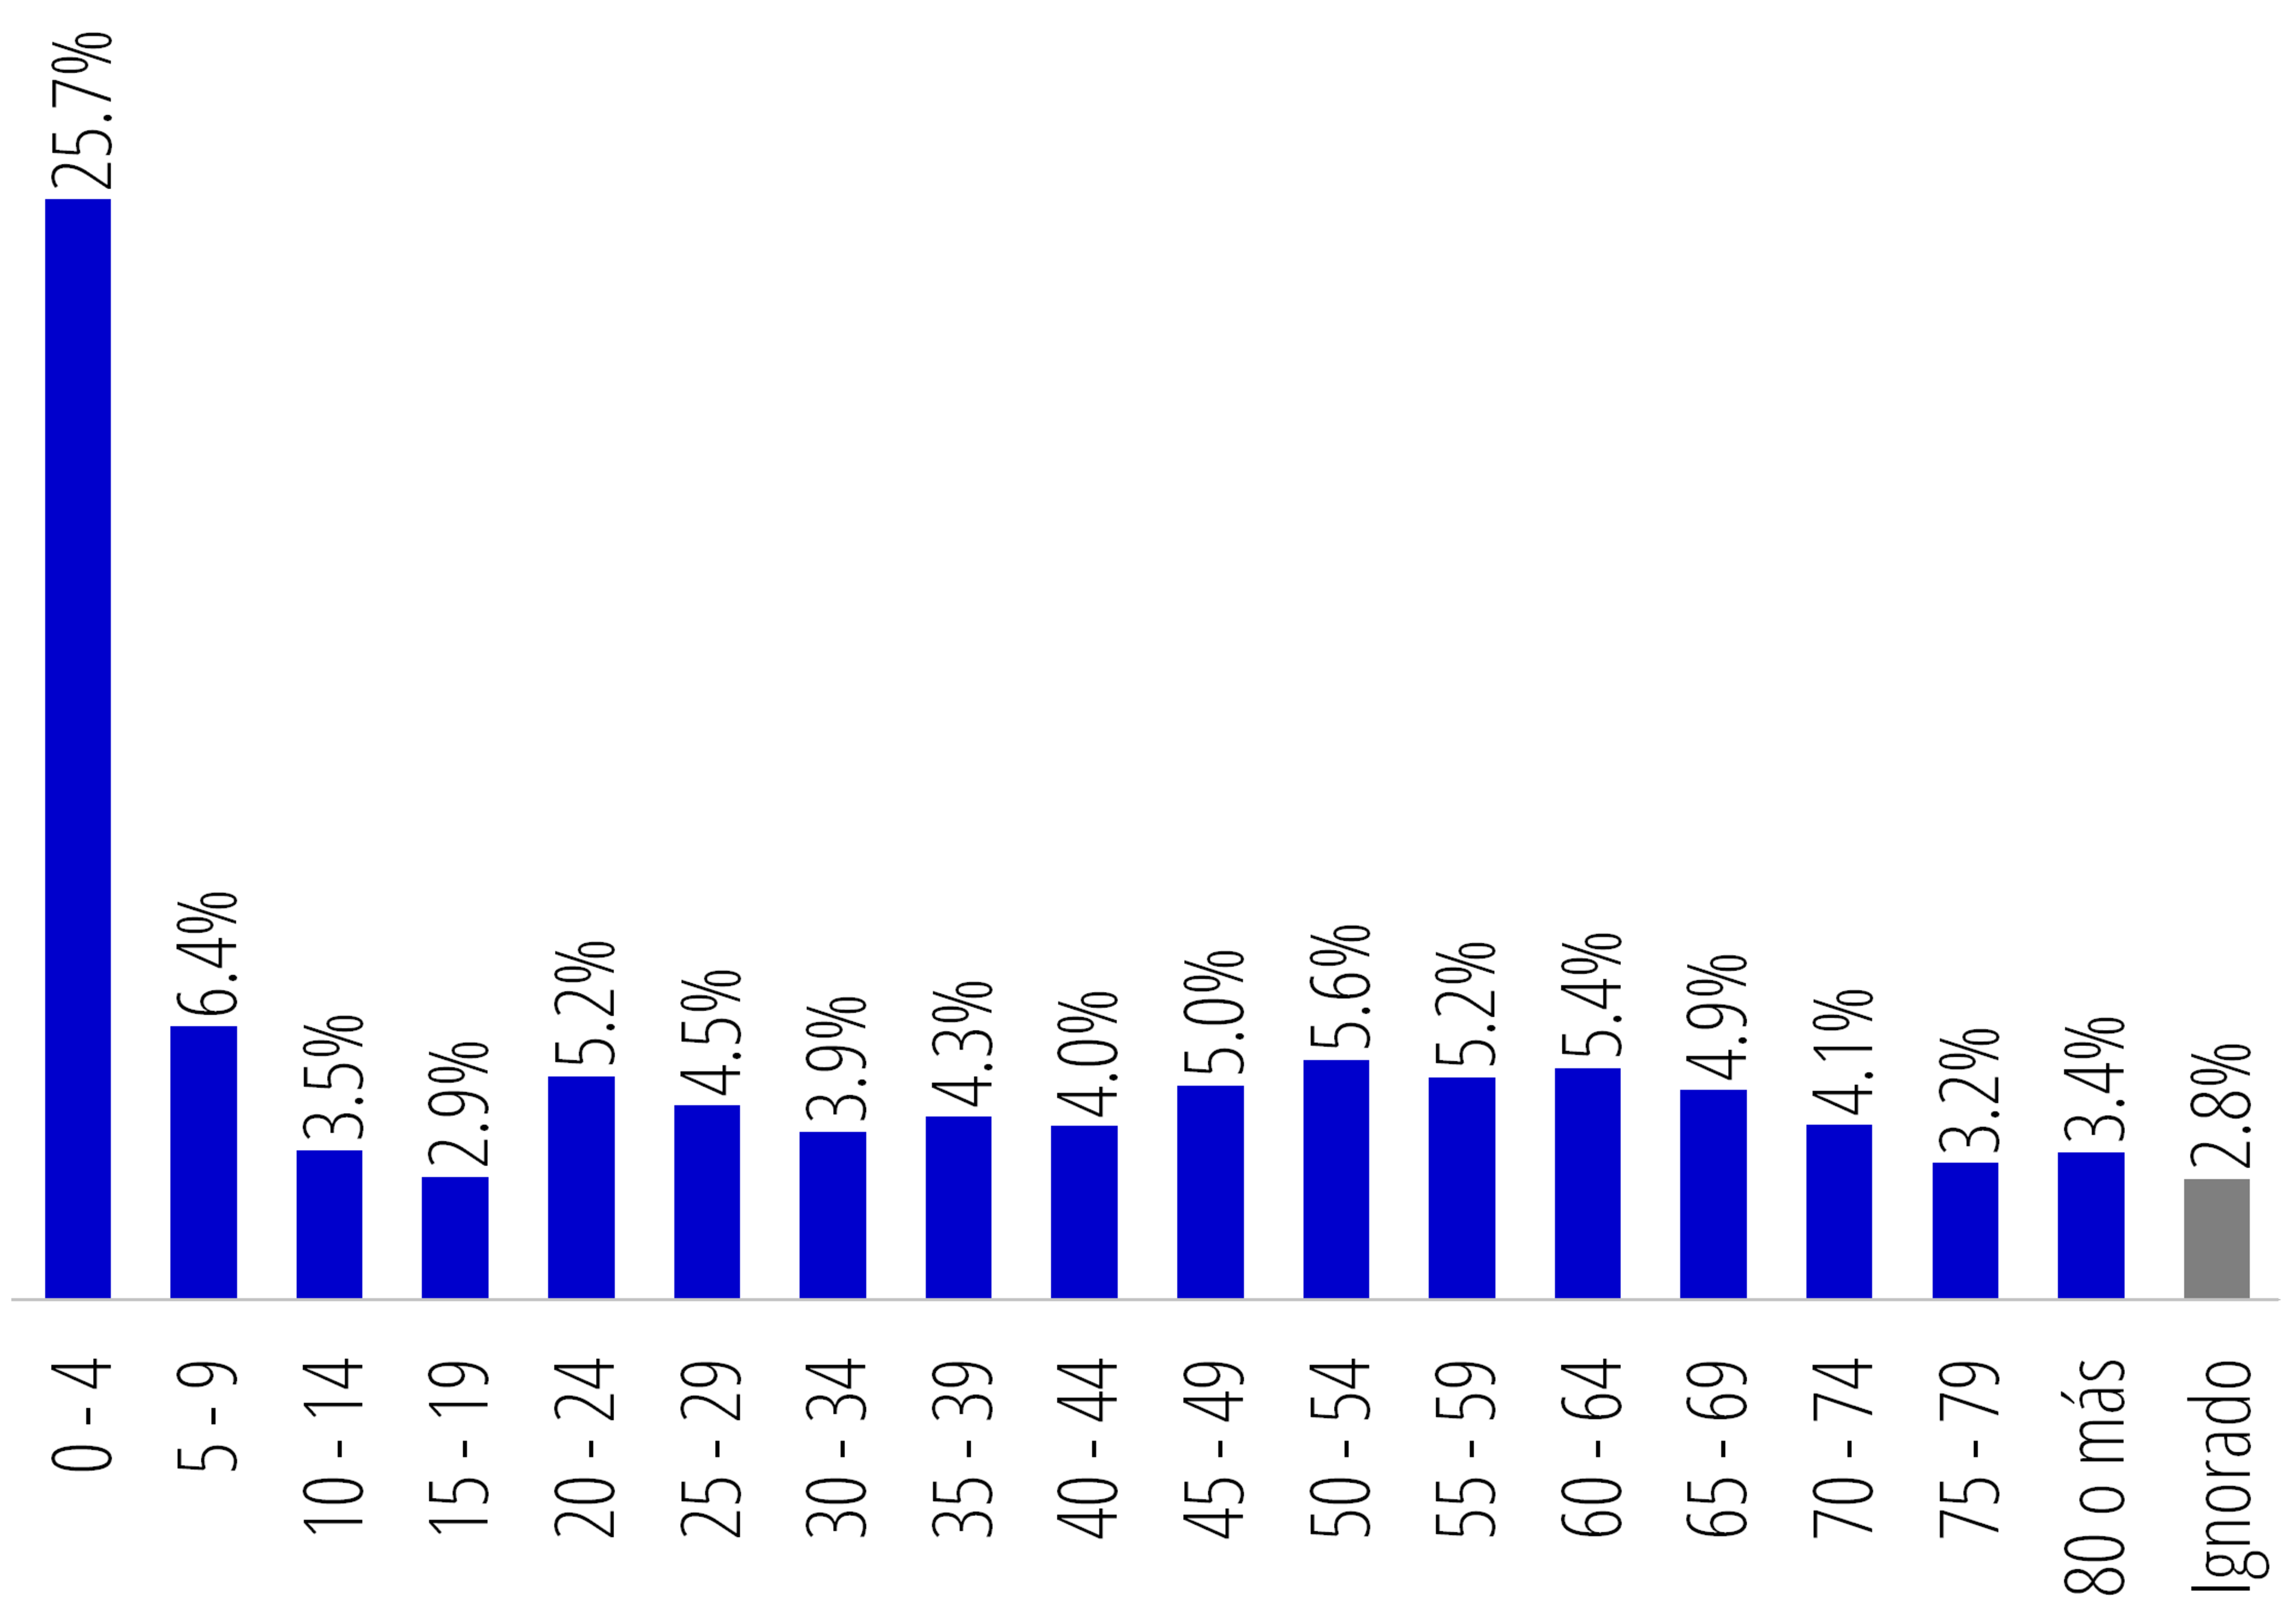
\includegraphics[width=32\cuadri]{plot.pdf}
\begin{flushleft}
$\ $\\[-2\cuadri]
\ \ \ \footnotesize Fuente: Estadísticas INE.
\end{flushleft}
\end{center}

\end{grafica-cajita}
\end{tabular}

\end{cajita-arriba}



\noindent\begin{cajita-abajo}
\stepcounter{section}
\addcontentsline{toc}{section}{\numberline{\thesection} Sección de prueba}
\titulizador{Sección de prueba, ésta también queremos que tenga un título largón para ver que ondas con las dobles cajas de título largo.}

\begin{tabular}[b]{@{}p{17.5\cuadri}@{}p{1.5\cuadri}@{} x{34\cuadri}@{}}
& &\\[0.5\cuadri]
\begin{descripcion-cajita}
\parskip 6pt\parindent 2em%
Hola, este es un ejemplo de párrafo.  Debo escribir algunas líneas para corroborar que separa los párrafos adecuadamente.  Esto resulta interesante.

Chaleco viteh\footnote{pruebitas que uno hace cuando tiene muchas ganas de aprender, hoho.  Vamos a hacer más pruebitas, y seguimos con las pruebitas} Ahora debo copiar y pegar el párrafo anterior, pero me da hueva.  Así que escribiré un poquito más. Continuando la discusión latinezca podemos\footnote{Ve, otra vez pasó esto.} apreciar que tengo mucho sueño.  Pero esto no es nada nuevo para el lector. Ahora debo copiar y pegar el párrafo anterior, pero me da hueva.

Hola, este es un ejemplo de párrafo.  Debo escribir algunas líneas para corroborar que separa los párrafos adecuadamente.  Esto resulta interesante.  Pero esto no es nada. 
\end{descripcion-cajita}
  & &
\begin{grafica-cajita}
\begin{center}
\textbf{Título de gráfica, veamos cómo se mira con dos líneas de largo, para ver el espacio en blanco.}\\[-1pt]
{\footnotesize\texttwelveudash$\,\,$Desagregación de gráfica$\,\,$\texttwelveudash}\\[0.6\cuadri]
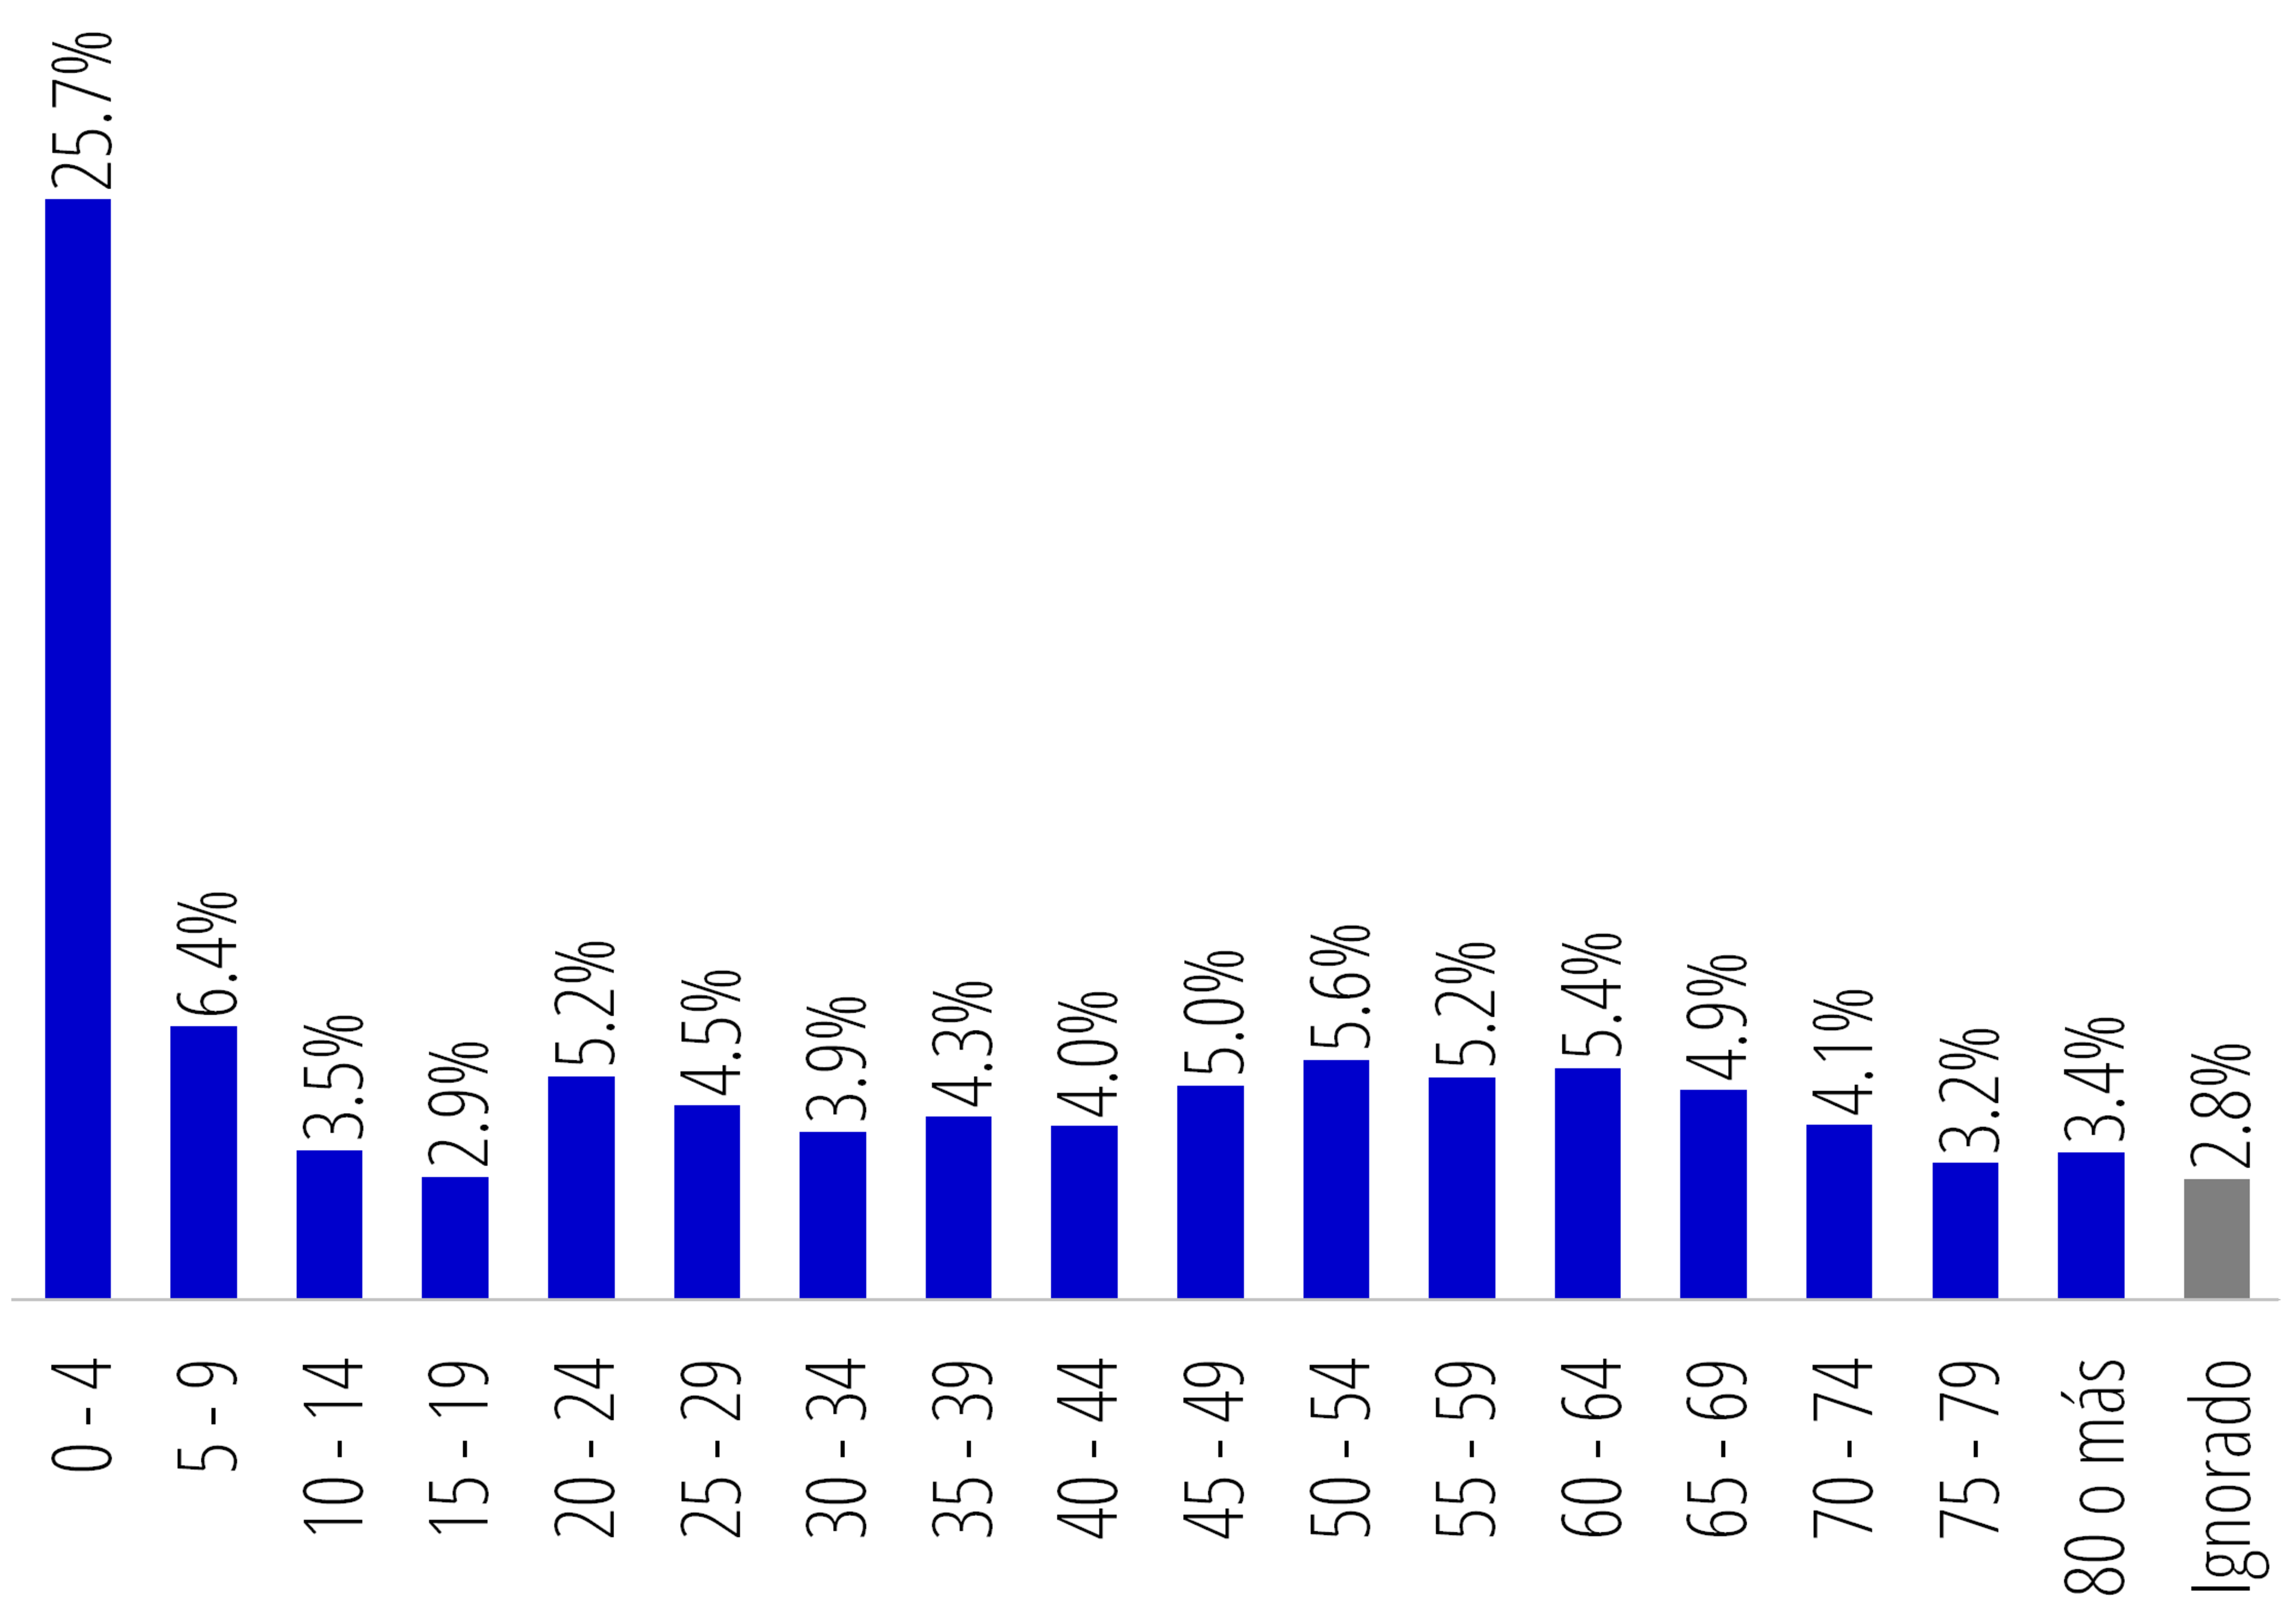
\includegraphics[width=32\cuadri]{plot.pdf}
\begin{flushleft}
$\ $\\[-2\cuadri]
\ \ \ \footnotesize Fuente: Estadísticas INE.
\end{flushleft}
\end{center}

\end{grafica-cajita}
\end{tabular}
\end{cajita-abajo}



\cajota{Título de caja largo wiri wiri Título de caja largo wiri wiri Título de caja largo wiri wiri }{\lipsum[4] hola\footnote{A ver dónde sale esto.  Esto es una nota sobre un mapa, estamos comprobando su localización final.  Pablito clavó un clavito en la calva de un calvito.  Una nota no muy larga podría verse extraña, esperemos que no sea así.} esto es una prueba de texto para ver qué pumas.  En teoría, la nota debería ser enviada hasta después de la gráfica, veamos si sucede lo que estoy prediciendo.}{Titulín de gráfica Titulín de gráfica Titulín de gráfica Titulín de gráfica Titulín de gráfica}{Desagregación de gráfica}{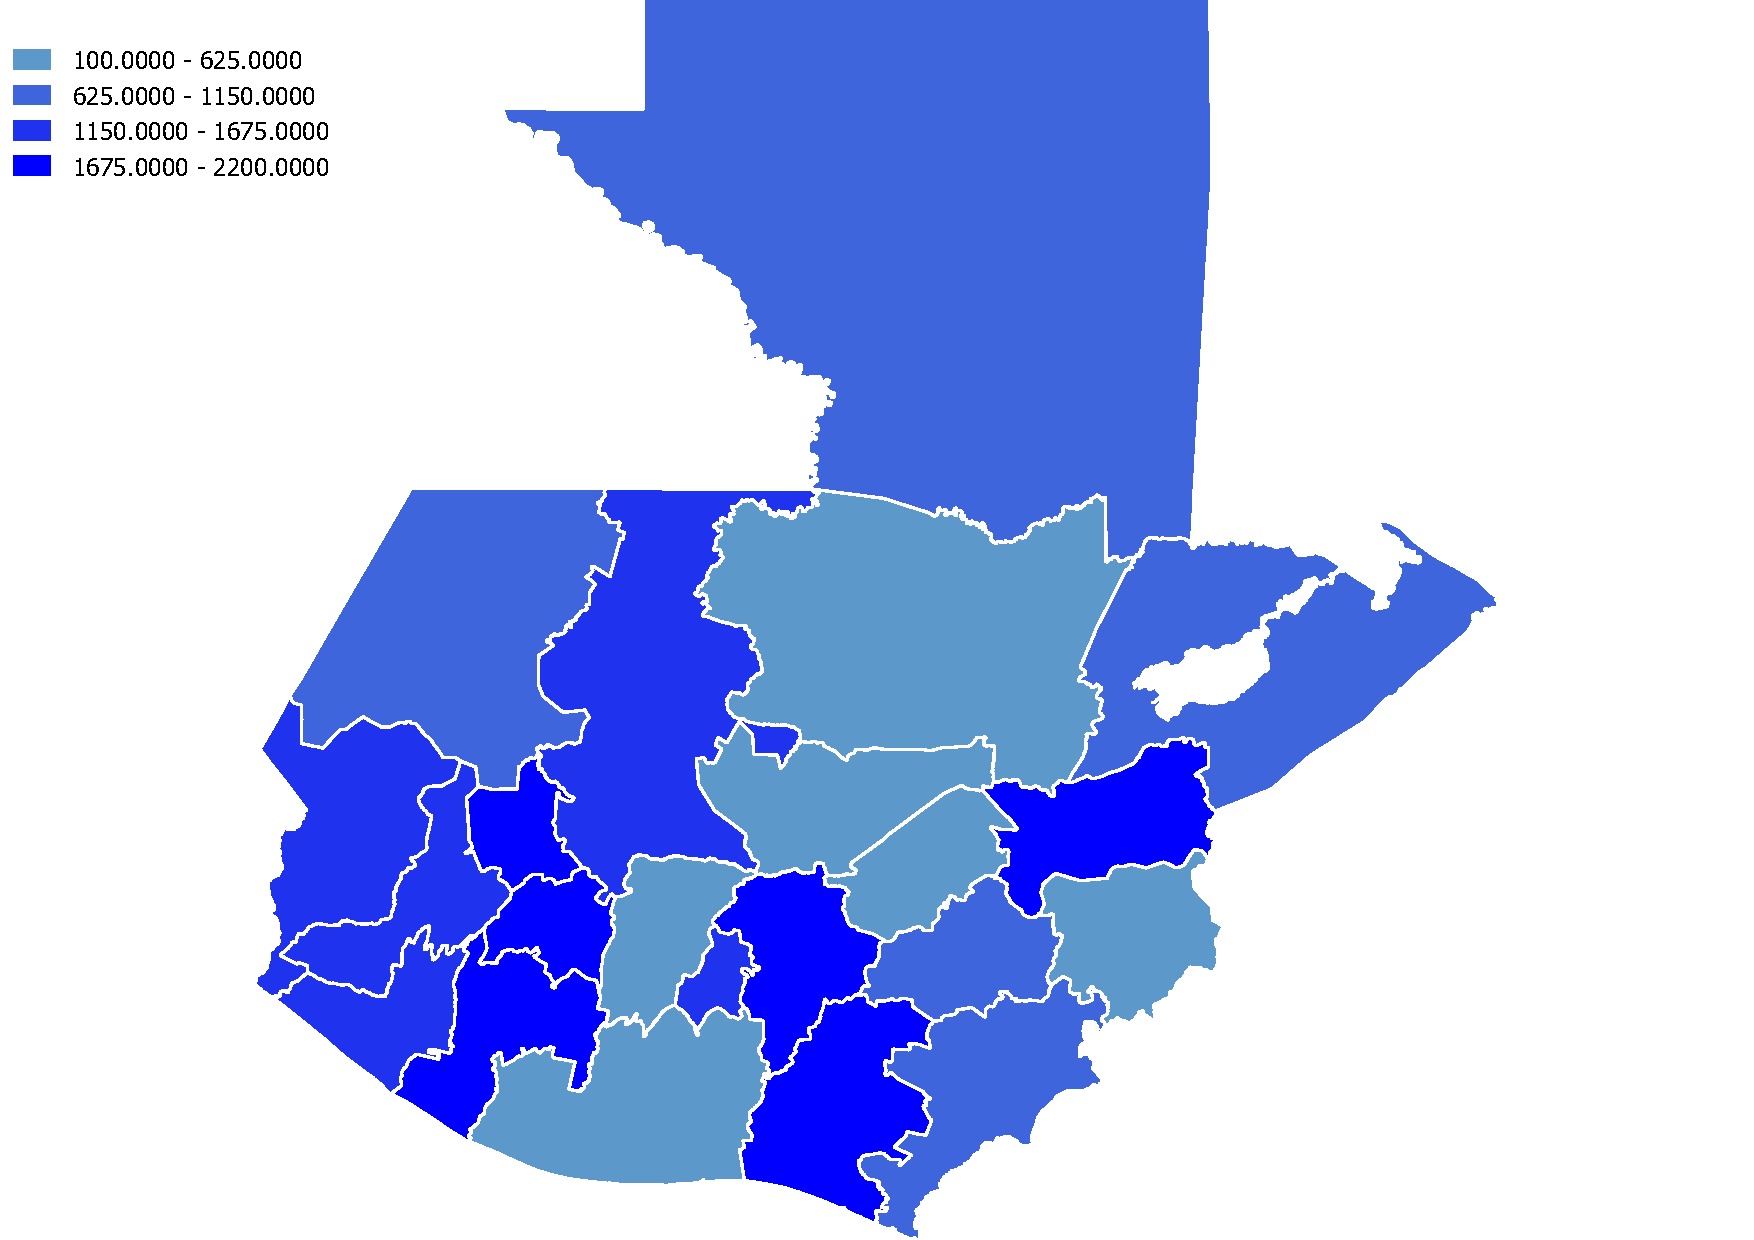
\includegraphics[width=52\cuadri]{mapa.pdf}}{Aquí va la fuente.}



\lipsum 





\lipsum \lipsum



\end{document}